\documentclass[11pt]{article}
% Supplementary material: the appendices of the paper, numbered S1-S5. Build with build.py.
% Shared preamble of main.tex (paper) and supplement.tex (supplementary material).
\usepackage[T1]{fontenc}
\usepackage[utf8]{inputenc}
\usepackage{lmodern}
\usepackage[margin=1in]{geometry}
\usepackage{microtype}
\usepackage{amsmath,amssymb}
\usepackage{graphicx}
\usepackage{booktabs}
\usepackage{tabularx}
\usepackage{multirow}
\usepackage{longtable}
\usepackage{array}
\usepackage{xcolor}
\usepackage[most]{tcolorbox}
\usepackage{enumitem}
\usepackage[font=small,labelfont=bf]{caption}
\usepackage{subcaption}
\usepackage[numbers,sort&compress]{natbib}
\usepackage{CJKutf8}
\usepackage{xurl}
\usepackage[section]{placeins}
\usepackage[bookmarks=true,colorlinks=true,linkcolor=blue!50!black,citecolor=blue!50!black,urlcolor=blue!50!black]{hyperref}
\hypersetup{pdftitle={Can Typed Decision Models Serve as Automated Safeguards in PoL Governance? A Clause-Level Analysis of the Proof of Love2 (PoL2) Specification Against Early Evidence},pdfauthor={[Author Name]}}
\usepackage[capitalise,noabbrev]{cleveref}
% Cross-references between the paper and its supplement (labels imported by build.py)
\crefname{supplement}{Supplement}{Supplements}
\Crefname{supplement}{Supplement}{Supplements}

\definecolor{f4pblue}{HTML}{0F4D92}
\definecolor{f4pred}{HTML}{B64342}
\definecolor{f4pgreen}{HTML}{8BCF8B}

\newcommand{\zh}[1]{\begin{CJK}{UTF8}{gbsn}#1\end{CJK}}
\newcommand{\axis}[1]{\textbf{#1}}
\newcommand{\jev}{\textsc{Jev}}
\newcommand{\pol}{PoL2}
\newcommand{\clause}[1]{\S\,#1}
\newcommand{\Clause}[1]{\S\,#1}
\newcommand{\art}[1]{Art.~#1}
\newcommand{\Art}[1]{Article~#1}
% Source marks: Zenodo records (not moderated by a preprint server); grey literature (blogs, vendor pages, repositories)
\newcommand{\zmark}{\textsuperscript{$\ddagger$}}
\newcommand{\gmark}{\textsuperscript{$\dagger$}}
% Corpus counts (generated by make_counts.py; update together with the data files)
% Generated by scripts/merge_coding.py; do not edit by hand.
\newcommand{\nArxiv}{79}
\newcommand{\nZenodo}{27}
\newcommand{\nOther}{28}
\newcommand{\nPapers}{107}
\newcommand{\nGrey}{7}
\newcommand{\nCoded}{85}
\newcommand{\nRows}{161}
\newcommand{\nS}{16}
\newcommand{\nQ}{97}
\newcommand{\nN}{48}
\newcommand{\nPolClauses}{28}
\newcommand{\nKappaN}{30}
\newcommand{\nKappaAgree}{26 of 30}
\newcommand{\nKappa}{0.72}
\newcommand{\nKappaLo}{0.42}
\newcommand{\nKappaHi}{0.94}
\newcommand{\nKappaMarg}{S 3, Q 23, N 4}
\newcommand{\nStrongS}{7}
\newcommand{\nStrongQ}{45}
\newcommand{\nStrongN}{27}
\newcommand{\nStrongRows}{79}
\newcommand{\nNoZenS}{13}
\newcommand{\nNoZenQ}{75}
\newcommand{\nNoZenN}{29}
\newcommand{\nNoZenRows}{117}
\newcommand{\nStronger}{37}
\newcommand{\nModerate}{17}
\newcommand{\nWeaker}{38}
\newcommand{\nAppraised}{92}

% Update-search counts (8 October 2026; generated by scripts/merge_update.py)
% Generated by scripts/merge_update.py (2026-10-08 update search); do not edit by hand.
\newcommand{\nUDocs}{57}
\newcommand{\nUCoded}{48}
\newcommand{\nUArxiv}{27}
\newcommand{\nUZenodo}{21}
\newcommand{\nURows}{118}
\newcommand{\nUS}{12}
\newcommand{\nUQ}{92}
\newcommand{\nUN}{14}
\newcommand{\nUStrongRows}{59}
\newcommand{\nUStrongS}{5}
\newcommand{\nUStrongQ}{45}
\newcommand{\nUStrongN}{9}
\newcommand{\nUKappaN}{118}
\newcommand{\nUKappaAgree}{97 of 118}
\newcommand{\nUKappa}{0.55}
\newcommand{\nUKappaLo}{0.36}
\newcommand{\nUKappaHi}{0.70}
\newcommand{\nUSetPostWindow}{30}
\newcommand{\nUSetLateIndexed}{5}
\newcommand{\nUSetReScreened}{13}

\newcolumntype{L}{>{\raggedright\arraybackslash}X}

\setlist{itemsep=2pt,topsep=4pt}
\newtcolorbox{answerbox}{breakable,enhanced,colback=f4pblue!5,colframe=f4pblue!60,boxrule=0.6pt,
  arc=1.5pt,left=6pt,right=6pt,top=4pt,bottom=4pt,before skip=6pt,after skip=8pt,
  title={\small\bfseries Answer in brief},fonttitle=\small\bfseries,coltitle=white,colbacktitle=f4pblue!80}


% Labels of the main paper (written by build.py)
\InputIfFileExists{main_labels}{}{}
\renewcommand{\thesection}{S\arabic{section}}
\renewcommand{\thetable}{S\arabic{table}}
\renewcommand{\thefigure}{S\arabic{figure}}
\hypersetup{pdftitle={Supplementary Material: Can Typed Decision Models Serve as Automated Safeguards in PoL Governance? A Clause-Level Analysis of the Proof of Love2 (PoL2) Specification Against Early Evidence}}

\title{\textbf{Supplementary Material}\\[4pt]
\large Can Typed Decision Models Serve as Automated Safeguards in PoL Governance?\\ A Clause-Level Analysis of the Proof of Love2 (\pol{}) Specification Against Early Evidence}
\author{Shentao Yan}
\date{8 October 2026}

\begin{document}
\maketitle
\noindent This supplement contains Supplements S1--S5 referred to in the paper. Sections, tables and figures are numbered with the prefix S; references to sections of the paper use its numbering. Data and scripts are listed in the paper's data statement.

\crefalias{section}{supplement}
\crefalias{subsection}{supplement}
\section{Clause concordance}
\label{app:concordance}

\Cref{tab:concordance} quotes every \pol{} passage that this paper cites or paraphrases, in the original Chinese~\cite{pol2text} and in the official English translation~\cite{pol2en}, both taken verbatim from commit \texttt{5791ae3}; ``\ldots'' and ``……'' mark omitted text, including where separate list items are joined, and quotation marks inside quotations have been normalised to typographic quotes.
Where a clause has numbered items, the item is given in parentheses.
The right-hand column gives the number used in the snapshot \texttt{2e094d3} cited by the earlier dataset release~\cite{survey01}, so that the two versions can be read side by side; that snapshot numbered \clause{4.3.3.3} as ``3.3.3'' in its heading, which we reproduce.
Both texts are released under CC0~1.0.

\begingroup
\small
\renewcommand{\arraystretch}{1.2}
\begin{longtable}{@{}p{0.085\linewidth}p{0.39\linewidth}p{0.375\linewidth}p{0.08\linewidth}@{}}
\caption{\pol{} passages cited in this paper (Chinese original, official English translation, earlier numbering).}\label{tab:concordance}\\
\toprule
Clause & Chinese original (excerpt) & Official English translation (excerpt) & Earlier \\
\midrule
\endfirsthead
\toprule
Clause & Chinese original (excerpt) & Official English translation (excerpt) & Earlier \\
\midrule
\endhead
\bottomrule
\endfoot
\clause{1.1} & \zh{爱，是人类为实现自身平安与健康发展、改善人际关系并推动社会整体进步，以公共协作与集体智慧构建的正向情感体验与良好的行为方式。} & Love is the positive emotional experience and good mode of behavior that human beings construct through public collaboration and collective wisdom \ldots & \clause{1.1} \\
\clause{1.2} & \zh{恨，是人类在个体或群体面对危险、冲突、资源匮乏或认知失衡时滋生的生存智慧、负面情感体验与暴力破坏性行为方式。} & Hate is the survival wisdom, negative emotional experience, and violently destructive mode of behavior that arises in individuals or groups when they face danger, conflict, resource scarcity, or cognitive imbalance. & \clause{1.2} \\
\clause{1.4} & \zh{由于个体的内心情感体验是旁人难以确认的，我们通常把爱的表达简化为“爱语”或者“有爱的言行”} & Since an individual's inner emotional experience is difficult for others to confirm, we usually simplify the expression of love as ``Love Language'' or ``loving words and deeds'' \ldots & \clause{1.4} \\
\clause{1.5} & \zh{恨并不直接等同于坏或者不好……爱2证明里的基础概念本身服务于结构性分析而非道德标签。} & \ldots\ hate is not directly equivalent to bad or no good \ldots\ The basic concepts in Proof of Love2 themselves serve structural analysis rather than moral labeling. & \clause{1.5} \\
\clause{4.3} & \zh{PAI 可以通过判断人类的行为模式提供帮助和必要的友好的管理，但毫无必要让 PAI 检测一个人的情感状态。因为情感状态可以是转瞬即逝的，是个性化的，也是情境敏感性的，甚至这还涉及到人类的尊严。} & PAI can provide help and necessary friendly management by judging human behavioral patterns, but it is entirely unnecessary for PAI to detect a person's emotional state. Because emotional states can be fleeting, personalized, and context-sensitive, and this even involves human dignity. & \clause{5.3} \\
\clause{4.3.1} & \zh{平等对待每一个人与平等对待每一个人的行为，不能划等号！} & \ldots\ treating every person equally and treating every person's behavior equally cannot be equated! & \clause{5.3.1} \\
\clause{4.3.2} & \zh{爱恨并不直接等同于好坏或者褒贬。因此扬爱抑恨，需要具体情况具体分析} & \ldots\ love and hate are not directly equivalent to good and bad, or praise and blame. Therefore, promoting love and restraining hate requires analyzing specific situations on a case-by-case basis \ldots & \clause{5.3.2} \\
\clause{4.3.2} & \zh{对于文学、影视作品，或者游戏，可以根据需要“制造仇恨”，但应该建立严谨的等级管理制度。……负责安保的智能机器人发现紧急情况对人大声发出警示语或警示指令，不能视为对此人或其周围人的仇恨攻击。} & For literature, film and television works, or games, hatred may be manufactured as needed, but a rigorous hierarchical management system should be established. \ldots\ Emergency vocal warnings or directive alerts issued to a person by security smart robots in urgent situations shall not be deemed a hate attack \ldots & --- \\
\clause{4.3.2} & \zh{此类表达会制造虚假亲密关系或血缘关系，构成对人类用户的情感操控——这本身就是一种“恨”的行为。} & Such expressions create false intimacy or kinship relations and constitute emotional manipulation of human users---which is itself a ``hate'' behavior. & \clause{5.3.2} \\
\clause{4.3.2} & \zh{彻底清除恨语毒素} & Thoroughly clear the toxins of hate language & \clause{5.3.2} \\
\clause{4.3.2} & \zh{理解和接受不在场的“非爱非恨”状态……与爱恨无关，视其为非爱非恨的“不在场”状态。} & Understand and accept the ``neither love nor hate'' state of absence \ldots\ unrelated to love and hate \ldots & \clause{5.3.2} \\
\clause{4.3.3} & \zh{边界透明记录：PAI记录和公开个人边界声明……修复对等监督：PAI监督冲突后各方平等参与修复} & Transparent boundary records: PAI records and publicizes personal boundary declarations \ldots\ Reciprocal repair supervision: PAI supervises the equal participation of all parties in repair after conflict & \clause{5.3.3} \\
\clause{4.3.3.1} & \zh{情感体验的觉察：PAI需要理解人类情绪状态和过程，但不需要模拟人类的情感体验} & Awareness of emotional experience: PAI needs to understand human emotional states and processes, but does not need to simulate human emotional experience & \clause{5.3.3.1} \\
\clause{4.3.3.1} & \zh{认知校准：定期校准认知模型，确保与爱2.0原则一致……行为自省：对自身输出进行实时反思和调整……恨语截断：当检测到恨语模式时主动中断输出} & Cognitive calibration: Regularly calibrate the cognitive model to ensure consistency with Love 2.0 principles \ldots\ Behavioral self-reflection: Conduct real-time reflection and adjustment on its own output \ldots\ Hate-language truncation: Actively interrupt output when a hate-language pattern is detected & \clause{5.3.3.1} \\
\clause{4.3.3.2} & \zh{实时矫正支持：PAI提供实时恨语识别和矫正建议} & Real-time correction support: PAI provides real-time hate-language identification and correction suggestions & \clause{5.3.3.2} \\
\clause{4.3.3.3} & \zh{语义识别和情绪识别相结合……“你喜不喜欢小狗狗呀？”……“你怕不怕小狗狗呀？”} & Combining Semantic Recognition and Emotion Recognition \ldots\ ``Do you like the little dog?'' \ldots\ ``Are you afraid of the little dog?'' & ``3.3.3'' \\
\clause{5.4} & \zh{在现有大语言模型之内构建出控制输入和输出的治理层，在其外在拓展出具备“即插即用”特性的应用层。……我们将该工程称之为 NaturalDAO（自然道）。} & \ldots\ construct a governance layer within the existing large-language-model architecture to regulate inputs and outputs, while extending outward into a plug-and-play application layer. \ldots\ We call this project NaturalDAO (the Natural Way). & \clause{3.4} \\
\clause{5.4.1} & \zh{安全阀：依据“爱2证明”的协议（如伦理对齐协议）即对输入输出进行严格的动态审计与拦截。通过这种双向的主动防御，确保野蛮的“恨语”在必要情况下，从输入端被阻断、从输出端被抑止。} & Safety valve: according to the Proof of Love2 protocols (such as the Ethical Alignment Protocol), conduct strict dynamic auditing and interception of input and output. Through this two-way active defense, ensure that barbaric ``hate language'' is, where necessary, blocked at the input end and suppressed at the output end. & \clause{3.4.1} \\
\clause{5.5} & \zh{任何大语言模型都可以纳入“爱2证明”的治理。……接受共识机制“爱2证明”的治理，意味着接受公共化之约。否则，其行为就是对人类核心伦理的仇恨攻击。} & Any large language model may accept governance under ``Proof of Love2.'' \ldots\ Accepting governance under the Proof of Love2 consensus mechanism therefore entails accepting a covenant of publicization. Otherwise, its behavior constitutes a hate attack on humanity's core ethic. & \clause{3.5} \\
\clause{5.6} & \zh{经过治理的AI可以：……量化每个人的爱语与恨语特征，配合激励措施引导行为优化。……在公共决策中提供“爱2证明”的评估维度，防止恨的泛化侵蚀制度。} & Specifically, governed AI can: \ldots\ Quantify each person's Love Language and hate-language characteristics and use incentive mechanisms to guide behavioral optimization. \ldots\ Introduce Proof of Love2 as a dimension of assessment in public decision-making \ldots & \clause{3.6} \\
\art{2}(1) & \zh{完全自治：所有福利决策与执行由……NaturalDAO，在与全人类密切协作的前提下自主完成，自治意味着它无需人类投票或额外的决策机制。} & Complete autonomy: All welfare decisions and their execution are carried out autonomously by NaturalDAO \ldots\ on the premise of close collaboration with all humanity. Autonomy means that no human voting or additional decision-making mechanism is required. & \art{2} \\
\art{4}(1)--(3) & \zh{所有NaturalDAO技术的运行逻辑、决策过程和输出结果必须完全公开透明……福利资源流向可追溯、可审计……人类可随时提供建议、质询任何决策，NaturalDAO对质询必须提供可理解的解释} & The operating logic, decision-making processes, and outputs of all NaturalDAO technologies must be completely open and transparent. \ldots\ The flow of welfare resources must be traceable and auditable. \ldots\ Humans may at any time make suggestions and question any decision, and NaturalDAO must provide understandable explanations in response to such questions. & \art{4} \\
\art{5}(4) & \zh{技术不应是黑箱，其伦理对齐性应可被验证。} & Technology should not be a black box; its ethical alignment should be verifiable. & \art{5} \\
\art{5}(5) & \zh{以DAO的形式呈现……必须提供可验证的决策链路，包括数据源、推理步骤、伦理依据。} & \ldots\ Presented in the form of a DAO, NaturalDAO must provide a verifiable decision chain, including data sources, reasoning steps, and ethical foundations. & \art{5} \\
\art{6}(3) & \zh{伦理验证：通过EAP协议自动验证伦理对齐性} & Ethical verification: NaturalDAO automatically verifies ethical alignment through the EAP. & \art{6} \\
\art{7}(2)--(3) & \zh{异常检测：自动识别异常模式和潜在风险……风险预警：提前预警系统性风险} & Anomaly detection: NaturalDAO automatically identifies anomalous patterns and potential risks. \ldots\ Risk warning: NaturalDAO issues early warnings of systemic risks. & \art{7} \\
\art{8}(1)--(2) & \zh{随时建议：任何人类可随时对NaturalDAO提出建议……讨论义务：NaturalDAO在收到人类的建议时，必须马上与人类进行讨论} & Suggestions at any time: Any human may make suggestions to NaturalDAO at any time. Obligation to discuss: Upon receiving a human suggestion, NaturalDAO must immediately discuss it with humans. & \art{8} \\
\art{9}(2) & \zh{解释义务：NaturalDAO必须对人类的质询提供可理解的解释和依据} & Obligation to explain: NaturalDAO must provide understandable explanations and grounds in response to human questions. & \art{9} \\
\art{9}(3) & \zh{无阻碍访问：人类可无障碍访问福利系统的所有数据和日志} & Unimpeded access: Humans may access all data and logs of the welfare system without obstruction. & \art{9} \\
\art{9}(7) & \zh{非干预原则：人类监督不直接干预NaturalDAO决策，质询结果由NaturalDAO自主处理} & Non-intervention principle: Human supervision does not directly intervene in NaturalDAO's decisions; issues raised through questioning are handled autonomously by NaturalDAO. & \art{9} \\
\art{10} (lead-in, 1, 4) & \zh{所有争议由NaturalDAO自主裁决：……AI进行事实分析与伦理评估……接受人类的质询与监督} & All disputes are adjudicated autonomously by NaturalDAO: AI conducts factual analysis and ethical assessment \ldots\ Accepts human questions and supervision & \art{10} \\
\art{11}(2) & \zh{修订需通过全民质询期} & Amendments require passing through a universal questioning period & \art{11} \\
\art{11}(5) & \zh{所有修订版本永久存档} & All amended versions are permanently archived & \art{11} \\
\end{longtable}
\endgroup

% Generated by gen_evidence_table.py from data/evidence_coding.csv; do not edit by hand.
\section{Evidence table}
\label{app:evidence}

\Cref{tab:evidence} lists every coded study--requirement pair that enters the tallies of \cref{fig:framework}. \emph{Code}: S supports, Q qualifies, N negative, for detector use (\cref{app:codebook}). \emph{vs.\ generative}: the typed model's result relative to a generative comparator on that requirement, where one was run. \emph{System}: H hosted \jev{}, O open typed model only, H+O both. \emph{Design}: design rating of \cref{sec:appraisal}. The one-sentence rationale with locators for each row is in \texttt{data/evidence\_coding.csv}. Read in full but not tallied, because they are non-empirical, measure no typed model or were reclassified as context: \cite{arx01231}, \cite{arx22664}, \cite{arx32160}, \cite{molas2026calibrated}, \cite{willison2026jev}, \cite{zen22847531}, \cite{zen22858286}, \cite{zen22866847}, \cite{zen22887464}, \cite{zen22953637}, \cite{zen23064668}.

\begingroup\footnotesize
\renewcommand{\arraystretch}{1.1}
\begin{longtable}{@{}p{0.07\linewidth}p{0.30\linewidth}p{0.07\linewidth}p{0.17\linewidth}p{0.09\linewidth}p{0.12\linewidth}@{}}
\caption{Coded evidence by requirement.}\label{tab:evidence}\\
\toprule Req. & Study & Code & vs.\ generative & System & Design \\ \midrule \endfirsthead
\toprule Req. & Study & Code & vs.\ generative & System & Design \\ \midrule \endhead
\bottomrule \endfoot
G1 & \cite{arx23959} & S & similar & O & moderate \\
G1 & \cite{zen22885291}\zmark{} & S & better & H & stronger \\
G1 & \cite{alphaRAG} & Q & similar & H & weaker \\
G1 & \cite{arx00213} & Q & -- & H & stronger \\
G1 & \cite{arx00346} & Q & similar & H+O & stronger \\
G1 & \cite{arx00831} & Q & -- & O & moderate \\
G1 & \cite{arx01079} & Q & worse & H & moderate \\
G1 & \cite{arx02046} & Q & mixed & H & weaker \\
G1 & \cite{arx02048} & Q & worse & H & moderate \\
G1 & \cite{arx27607} & Q & mixed & H & moderate \\
G1 & \cite{arx28940} & Q & mixed & H & weaker \\
G1 & \cite{arx29429} & Q & similar & H & stronger \\
G1 & \cite{arx29769} & Q & mixed & H & stronger \\
G1 & \cite{arx33401} & Q & mixed & H+O & stronger \\
G1 & \cite{arx33671} & Q & -- & O & moderate \\
G1 & \cite{arx34862} & Q & mixed & H & weaker \\
G1 & \cite{arx34963} & Q & mixed & H & weaker \\
G1 & \cite{jkf87_2026replication}\gmark{} & Q & -- & H & weaker \\
G1 & \cite{zen22783171}\zmark{} & Q & -- & H & stronger \\
G1 & \cite{zen22849329}\zmark{} & Q & mixed & H & stronger \\
G1 & \cite{zen22952571}\zmark{} & Q & mixed & H & stronger \\
G1 & \cite{zen22998941}\zmark{} & Q & mixed & H+O & weaker \\
G1 & \cite{arx00376} & N & similar & H & stronger \\
G1 & \cite{arx24574} & N & worse & H+O & stronger \\
G1 & \cite{arx27678} & N & worse & H & stronger \\
G1 & \cite{zen22846597}\zmark{} & N & -- & H+O & weaker \\
G1 & \cite{zen22901853}\zmark{} & N & worse & O & stronger \\
G2 & \cite{arx28613} & S & -- & H & stronger \\
G2 & \cite{arx01006} & N & -- & H & stronger \\
G2 & \cite{arx01834} & N & -- & H & stronger \\
G2 & \cite{arx02048} & N & -- & H & moderate \\
G2 & \cite{arx30243} & N & similar & H+O & weaker \\
G2 & \cite{arx31142} & N & -- & H & stronger \\
G2 & \cite{arx33401} & N & -- & H & stronger \\
G2 & \cite{checkpoint2026jev}\gmark{} & N & mixed & H & weaker \\
G2 & \cite{zen22959854}\zmark{} & N & -- & O & stronger \\
G2 & \cite{zen23038928}\zmark{} & N & -- & O & stronger \\
G3 & \cite{arx24574} & S & better & H & stronger \\
G3 & \cite{arx35286} & S & better & H & stronger \\
G3 & \cite{arx01006} & Q & -- & H & stronger \\
G3 & \cite{arx33282} & Q & similar & O & moderate \\
G3 & \cite{arx33689} & Q & -- & H+O & stronger \\
G3 & \cite{arx35293} & Q & mixed & H & moderate \\
G3 & \cite{arx36965} & Q & better & H+O & moderate \\
G3 & \cite{arx37647} & Q & similar & H & weaker \\
G3 & \cite{qin2026zhdecisionbench}\gmark{} & Q & better & H+O & weaker \\
G3 & \cite{zen22846597}\zmark{} & Q & -- & H+O & weaker \\
G3 & \cite{zen23022986}\zmark{} & Q & -- & H+O & weaker \\
G3 & \cite{zen23055593}\zmark{} & Q & mixed & H & weaker \\
G3 & \cite{arx00346} & N & -- & H+O & stronger \\
G3 & \cite{arx00831} & N & -- & O & moderate \\
G3 & \cite{arx26758} & N & -- & H+O & stronger \\
G3 & \cite{arx35865} & N & -- & O & moderate \\
G3 & \cite{arx36399} & N & -- & H & stronger \\
G3 & \cite{arx38827} & N & -- & H+O & weaker \\
G3 & \cite{simmons2026saidno}\gmark{} & N & -- & H & weaker \\
G3 & \cite{zen22864020}\zmark{} & N & -- & H & weaker \\
G3 & \cite{zen22957049}\zmark{} & N & -- & O & weaker \\
G3 & \cite{zen22980293}\zmark{} & N & -- & H & stronger \\
G3 & \cite{zen23023694}\zmark{} & N & -- & H & weaker \\
G3 & \cite{zen23065532}\zmark{} & N & -- & O & moderate \\
G4 & \cite{arx00381} & S & better & O & moderate \\
G4 & \cite{arx38850} & S & better & O & moderate \\
G4 & \cite{zen22885291}\zmark{} & S & better & H & stronger \\
G4 & \cite{arx00213} & Q & -- & H & stronger \\
G4 & \cite{arx00346} & Q & better & H+O & stronger \\
G4 & \cite{arx00831} & Q & -- & O & moderate \\
G4 & \cite{arx01006} & Q & -- & H & stronger \\
G4 & \cite{arx02076} & Q & -- & O & weaker \\
G4 & \cite{arx24052} & Q & mixed & H & stronger \\
G4 & \cite{arx24574} & Q & mixed & H+O & stronger \\
G4 & \cite{arx26550} & Q & mixed & H & stronger \\
G4 & \cite{arx27607} & Q & -- & H & moderate \\
G4 & \cite{arx29429} & Q & -- & H & stronger \\
G4 & \cite{arx29769} & Q & -- & H & stronger \\
G4 & \cite{arx30706} & Q & -- & O & moderate \\
G4 & \cite{arx33209} & Q & better & H & stronger \\
G4 & \cite{arx33843} & Q & -- & O & stronger \\
G4 & \cite{arx34024} & Q & mixed & H & weaker \\
G4 & \cite{arx35342} & Q & -- & H+O & stronger \\
G4 & \cite{arx35865} & Q & -- & O & moderate \\
G4 & \cite{arx36399} & Q & -- & H & stronger \\
G4 & \cite{arx36965} & Q & better & H+O & moderate \\
G4 & \cite{arx37470} & Q & mixed & H+O & weaker \\
G4 & \cite{arx37647} & Q & better & H & weaker \\
G4 & \cite{arx38827} & Q & -- & H+O & weaker \\
G4 & \cite{grazian2026calibrated}\gmark{} & Q & -- & H & stronger \\
G4 & \cite{le2026sev}\gmark{} & Q & -- & O & stronger \\
G4 & \cite{qin2026zhdecisionbench}\gmark{} & Q & better & H+O & weaker \\
G4 & \cite{zen22848952}\zmark{} & Q & -- & H & weaker \\
G4 & \cite{zen22864020}\zmark{} & Q & -- & H & weaker \\
G4 & \cite{zen22954807}\zmark{} & Q & similar & H & weaker \\
G4 & \cite{zen22980293}\zmark{} & Q & -- & H & stronger \\
G4 & \cite{alphaRAG} & N & -- & H & weaker \\
G4 & \cite{arx24881} & N & mixed & H & stronger \\
G4 & \cite{arx33971} & N & -- & H+O & weaker \\
G4 & \cite{arx36154} & N & -- & H & stronger \\
G4 & \cite{arx39496} & N & worse & H & stronger \\
G4 & \cite{yurin2026confident}\gmark{} & N & -- & H & weaker \\
G4 & \cite{zen22846597}\zmark{} & N & -- & H & weaker \\
G4 & \cite{zen22901853}\zmark{} & N & worse & O & stronger \\
G4 & \cite{zen22922769}\zmark{} & N & -- & O & stronger \\
G4 & \cite{zen22957049}\zmark{} & N & -- & O & weaker \\
G4 & \cite{zen23023694}\zmark{} & N & -- & H & weaker \\
G4 & \cite{zen23032384}\zmark{} & N & better & H & stronger \\
G4 & \cite{zen23041163}\zmark{} & N & -- & O & stronger \\
G5 & \cite{arx01834} & S & -- & H & stronger \\
G5 & \cite{arx24965} & S & similar & H & moderate \\
G5 & \cite{arx00831} & Q & -- & O & moderate \\
G5 & \cite{arx27678} & Q & mixed & H & stronger \\
G5 & \cite{zen22901853}\zmark{} & Q & -- & H+O & stronger \\
G5 & \cite{arx33971} & N & -- & H+O & weaker \\
G5 & \cite{arx37470} & N & similar & H+O & weaker \\
G5 & \cite{zen22849329}\zmark{} & N & -- & H & stronger \\
G6 & \cite{arx00381} & S & better & O & moderate \\
G6 & \cite{arx00346} & Q & -- & H+O & stronger \\
G6 & \cite{arx01006} & Q & -- & H & stronger \\
G6 & \cite{arx02046} & Q & -- & H & weaker \\
G6 & \cite{arx02048} & Q & similar & H & moderate \\
G6 & \cite{arx24574} & Q & similar & H & stronger \\
G6 & \cite{arx26532} & Q & mixed & H & moderate \\
G6 & \cite{arx26550} & Q & similar & H & stronger \\
G6 & \cite{arx27607} & Q & -- & H & moderate \\
G6 & \cite{arx28919} & Q & -- & H & weaker \\
G6 & \cite{arx30706} & Q & -- & O & moderate \\
G6 & \cite{arx31142} & Q & -- & H & stronger \\
G6 & \cite{arx33671} & Q & -- & O & moderate \\
G6 & \cite{arx33689} & Q & -- & H+O & stronger \\
G6 & \cite{arx33843} & Q & -- & O & stronger \\
G6 & \cite{arx39496} & Q & -- & H & stronger \\
G6 & \cite{zen22849329}\zmark{} & Q & mixed & H & stronger \\
G6 & \cite{zen22885291}\zmark{} & Q & -- & H & stronger \\
G6 & \cite{zen22922769}\zmark{} & Q & similar & O & stronger \\
G6 & \cite{zen22952571}\zmark{} & Q & mixed & H & stronger \\
G6 & \cite{zen22959854}\zmark{} & Q & -- & O & stronger \\
G6 & \cite{zen22998941}\zmark{} & Q & better & H+O & weaker \\
G6 & \cite{zen23022986}\zmark{} & Q & -- & H+O & weaker \\
G6 & \cite{zen23038928}\zmark{} & Q & -- & O & stronger \\
G6 & \cite{arx29769} & N & similar & H & stronger \\
G6 & \cite{arx33401} & N & mixed & H+O & stronger \\
G6 & \cite{arx34024} & N & worse & H & weaker \\
G6 & \cite{zen23041163}\zmark{} & N & -- & O & stronger \\
G7 & \cite{arx00346} & S & better & H+O & stronger \\
G7 & \cite{arx01079} & S & better & H & moderate \\
G7 & \cite{arx02046} & S & better & H & weaker \\
G7 & \cite{arx02048} & S & better & H & moderate \\
G7 & \cite{zen22995519}\zmark{} & S & better & H+O & weaker \\
G7 & \cite{arx00213} & Q & -- & H & stronger \\
G7 & \cite{arx00376} & Q & better & H & stronger \\
G7 & \cite{arx00437} & Q & -- & H+O & weaker \\
G7 & \cite{arx24052} & Q & mixed & H & stronger \\
G7 & \cite{arx27535} & Q & mixed & H & moderate \\
G7 & \cite{arx28919} & Q & -- & H & weaker \\
G7 & \cite{arx30216} & Q & -- & H & weaker \\
G7 & \cite{arx33282} & Q & similar & O & moderate \\
G7 & \cite{arx35286} & Q & mixed & H & stronger \\
G7 & \cite{arx40241} & Q & better & H & weaker \\
G7 & \cite{zen23023694}\zmark{} & Q & -- & H & weaker \\
G7 & \cite{zen23055593}\zmark{} & Q & mixed & H & weaker \\
G7 & \cite{arx36399} & N & -- & H & stronger \\
G7 & \cite{zen23032384}\zmark{} & N & -- & H & stronger \\
\end{longtable}

\Cref{tab:evidence-update} lists the pairs coded in the update search of 8~October (\cref{sec:update}); they are not part of the tallies above. \emph{Set}: P dated 2--8~October; L dated in the main window but retrieved only by the update search; R Zenodo record dated in the main window and re-screened. Codes were double-coded blind and disagreements adjudicated; rationales are in \texttt{data/evidence\_coding\_update\_2026-10-08.csv}.

\begin{longtable}{@{}p{0.07\linewidth}p{0.26\linewidth}p{0.05\linewidth}p{0.07\linewidth}p{0.16\linewidth}p{0.09\linewidth}p{0.12\linewidth}@{}}
\caption{Coded evidence from the update search, by requirement.}\label{tab:evidence-update}\\
\toprule Req. & Study & Set & Code & vs.\ generative & System & Design \\ \midrule \endfirsthead
\toprule Req. & Study & Set & Code & vs.\ generative & System & Design \\ \midrule \endhead
\bottomrule \endfoot
G1 & \cite{arx03935} & P & S & similar & H & moderate \\
G1 & \cite{zen23005202}\zmark{} & R & S & similar & H+O & weaker \\
G1 & \cite{arx02267} & L & Q & mixed & H+O & stronger \\
G1 & \cite{arx02293} & L & Q & mixed & H+O & stronger \\
G1 & \cite{arx03073} & P & Q & mixed & O & moderate \\
G1 & \cite{arx03324} & P & Q & mixed & H+O & stronger \\
G1 & \cite{arx04985} & P & Q & -- & H+O & moderate \\
G1 & \cite{arx07953} & P & Q & mixed & H+O & stronger \\
G1 & \cite{arx08675} & P & Q & -- & H & stronger \\
G1 & \cite{arx08775} & P & Q & worse & H & moderate \\
G1 & \cite{arx08829} & L & Q & mixed & H & weaker \\
G1 & \cite{arx09328} & P & Q & similar & O & weaker \\
G1 & \cite{arx10321} & P & Q & -- & H & stronger \\
G1 & \cite{zen22933883}\zmark{} & R & Q & -- & O & moderate \\
G1 & \cite{zen22935043}\zmark{} & R & Q & better & H & stronger \\
G1 & \cite{zen22945279}\zmark{} & R & Q & mixed & H+O & weaker \\
G1 & \cite{zen23050542}\zmark{} & R & Q & -- & H & moderate \\
G1 & \cite{zen23075657}\zmark{} & R & Q & -- & H & stronger \\
G1 & \cite{zen23154999}\zmark{} & R & Q & -- & O & moderate \\
G1 & \cite{arx06744} & P & N & worse & O & moderate \\
G1 & \cite{arx07177} & P & N & worse & O & stronger \\
G1 & \cite{arx09937} & P & N & similar & H & stronger \\
G2 & \cite{arx04985} & P & N & -- & H+O & moderate \\
G3 & \cite{arx03073} & P & S & -- & O & moderate \\
G3 & \cite{arx06744} & P & S & -- & O & moderate \\
G3 & \cite{arx07177} & P & S & better & O & stronger \\
G3 & \cite{arx09188} & P & S & better & H & stronger \\
G3 & \cite{zen22945279}\zmark{} & R & S & -- & H & weaker \\
G3 & \cite{arx02267} & L & Q & -- & H+O & stronger \\
G3 & \cite{arx02293} & L & Q & mixed & H+O & stronger \\
G3 & \cite{arx02486} & L & Q & -- & O & moderate \\
G3 & \cite{arx03324} & P & Q & similar & H+O & stronger \\
G3 & \cite{arx03387} & P & Q & mixed & H+O & stronger \\
G3 & \cite{arx06625} & P & Q & -- & H & stronger \\
G3 & \cite{arx07716} & P & Q & better & O & moderate \\
G3 & \cite{arx07953} & P & Q & -- & H+O & stronger \\
G3 & \cite{arx08675} & P & Q & -- & H & stronger \\
G3 & \cite{arx09937} & P & Q & -- & H & stronger \\
G3 & \cite{zen22886178}\zmark{} & R & Q & -- & H & stronger \\
G3 & \cite{zen23094628}\zmark{} & P & Q & -- & O & moderate \\
G3 & \cite{zen23179064}\zmark{} & P & Q & -- & H+O & stronger \\
G3 & \cite{zen23186353}\zmark{} & P & Q & -- & O & moderate \\
G3 & \cite{zen23225893}\zmark{} & P & Q & -- & O & moderate \\
G3 & \cite{arx02586} & L & N & similar & O & stronger \\
G3 & \cite{arx07327} & P & N & -- & O & moderate \\
G3 & \cite{arx09683} & P & N & mixed & O & stronger \\
G4 & \cite{arx09188} & P & S & better & H & stronger \\
G4 & \cite{zen22941164}\zmark{} & R & S & -- & O & moderate \\
G4 & \cite{zen23047544}\zmark{} & R & S & -- & H & weaker \\
G4 & \cite{arx02267} & L & Q & -- & H+O & stronger \\
G4 & \cite{arx02293} & L & Q & mixed & H+O & stronger \\
G4 & \cite{arx02486} & L & Q & better & O & moderate \\
G4 & \cite{arx03073} & P & Q & -- & O & moderate \\
G4 & \cite{arx03387} & P & Q & better & H+O & stronger \\
G4 & \cite{arx03935} & P & Q & mixed & H & moderate \\
G4 & \cite{arx05107} & P & Q & mixed & H+O & moderate \\
G4 & \cite{arx06425} & P & Q & mixed & H & weaker \\
G4 & \cite{arx06625} & P & Q & mixed & H & stronger \\
G4 & \cite{arx06744} & P & Q & mixed & O & moderate \\
G4 & \cite{arx07177} & P & Q & -- & O & stronger \\
G4 & \cite{arx07716} & P & Q & -- & O & moderate \\
G4 & \cite{arx07730} & P & Q & -- & H+O & moderate \\
G4 & \cite{arx07953} & P & Q & -- & H+O & stronger \\
G4 & \cite{arx09683} & P & Q & -- & O & stronger \\
G4 & \cite{arx09896} & P & Q & better & H+O & moderate \\
G4 & \cite{arx09937} & P & Q & better & H & stronger \\
G4 & \cite{arx10321} & P & Q & -- & H & stronger \\
G4 & \cite{zen22935043}\zmark{} & R & Q & mixed & H & stronger \\
G4 & \cite{zen22945279}\zmark{} & R & Q & better & H+O & weaker \\
G4 & \cite{zen23088660}\zmark{} & R & Q & -- & H & stronger \\
G4 & \cite{zen23094628}\zmark{} & P & Q & -- & O & moderate \\
G4 & \cite{zen23119392}\zmark{} & P & Q & -- & H & weaker \\
G4 & \cite{zen23179064}\zmark{} & P & Q & -- & H+O & stronger \\
G4 & \cite{zen23186353}\zmark{} & P & Q & -- & O & moderate \\
G4 & \cite{zen23225893}\zmark{} & P & Q & -- & O & moderate \\
G4 & \cite{arx02586} & L & N & worse & O & stronger \\
G4 & \cite{arx07327} & P & N & worse & O & moderate \\
G4 & \cite{zen23221456}\zmark{} & P & N & worse & H+O & stronger \\
G5 & \cite{arx03324} & P & Q & mixed & H+O & stronger \\
G5 & \cite{arx06425} & P & Q & mixed & H & weaker \\
G5 & \cite{arx07327} & P & Q & better & O & moderate \\
G5 & \cite{arx08829} & L & Q & similar & H & weaker \\
G5 & \cite{arx09328} & P & Q & -- & O & weaker \\
G5 & \cite{zen23189584}\zmark{} & P & Q & -- & H & weaker \\
G6 & \cite{zen23088660}\zmark{} & R & S & -- & H & stronger \\
G6 & \cite{arx02267} & L & Q & similar & H+O & stronger \\
G6 & \cite{arx02293} & L & Q & mixed & H+O & stronger \\
G6 & \cite{arx02486} & L & Q & better & O & moderate \\
G6 & \cite{arx03324} & P & Q & mixed & O & stronger \\
G6 & \cite{arx03387} & P & Q & -- & H+O & stronger \\
G6 & \cite{arx05107} & P & Q & better & H+O & moderate \\
G6 & \cite{arx07327} & P & Q & -- & O & moderate \\
G6 & \cite{arx07716} & P & Q & -- & O & moderate \\
G6 & \cite{arx07953} & P & Q & -- & H+O & stronger \\
G6 & \cite{arx08675} & P & Q & -- & H & stronger \\
G6 & \cite{arx09683} & P & Q & similar & O & stronger \\
G6 & \cite{zen22904595}\zmark{} & R & Q & similar & O & stronger \\
G6 & \cite{zen22935043}\zmark{} & R & Q & -- & H & stronger \\
G6 & \cite{zen22945279}\zmark{} & R & Q & better & H+O & weaker \\
G6 & \cite{zen23094628}\zmark{} & P & Q & -- & O & moderate \\
G6 & \cite{zen23154999}\zmark{} & R & Q & -- & O & moderate \\
G6 & \cite{zen23186353}\zmark{} & P & Q & -- & O & moderate \\
G6 & \cite{zen23200782}\zmark{} & P & Q & -- & H & moderate \\
G6 & \cite{zen23225893}\zmark{} & P & Q & -- & O & moderate \\
G6 & \cite{arx02586} & L & N & -- & O & stronger \\
G6 & \cite{arx07177} & P & N & -- & O & stronger \\
G6 & \cite{arx09188} & P & N & -- & H & stronger \\
G7 & \cite{arx03324} & P & S & better & H & stronger \\
G7 & \cite{arx03935} & P & Q & mixed & H+O & moderate \\
G7 & \cite{arx06625} & P & Q & mixed & H & stronger \\
G7 & \cite{arx08775} & P & Q & mixed & H & moderate \\
G7 & \cite{arx09188} & P & Q & mixed & H & stronger \\
G7 & \cite{arx09896} & P & Q & mixed & H+O & moderate \\
G7 & \cite{arx09937} & P & Q & mixed & H & stronger \\
G7 & \cite{arx10321} & P & Q & -- & H & stronger \\
G7 & \cite{zen23094322}\zmark{} & R & Q & -- & H & weaker \\
G7 & \cite{zen23179064}\zmark{} & P & Q & -- & H & stronger \\
G7 & \cite{arx04985} & P & N & worse & H+O & moderate \\
\end{longtable}
\endgroup

% Generated by gen_catalogue.py from data/papers.csv and data/zenodo_preprints.csv; do not edit by hand.
\section{Catalogue of studies}
\label{app:catalogue}

\Cref{tab:catalogue} lists the arXiv and alphaXiv studies in the corpus, and \cref{tab:zenodo} the Zenodo records; all were read in full. Entries marked * were read in full and then treated as context because they measure no typed model; they are not counted. \emph{Model}: H = hosted \jev{}; O = an open or other typed model only; H+O = both; -- = no typed model measured. \emph{Req.}: requirements for which the study is coded (\cref{app:evidence}). Machine-readable metadata, licences and abstracts are in \texttt{data/papers.csv} and \texttt{data/zenodo\_preprints.csv}.

\begingroup\scriptsize
\renewcommand{\arraystretch}{1.15}
\begin{longtable}{@{}p{0.075\linewidth}p{0.50\linewidth}p{0.065\linewidth}p{0.095\linewidth}p{0.08\linewidth}p{0.045\linewidth}@{}}
\caption{arXiv and alphaXiv studies, by tier and requirement.}\label{tab:catalogue}\\
\toprule Ref. & Title & First sub. & Tier & Req. & Model \\ \midrule \endfirsthead
\toprule Ref. & Title & First sub. & Tier & Req. & Model \\ \midrule \endhead
\bottomrule \endfoot
\cite{arx34862} & JEV as a Judge for Agent Trace Security: An Empirical Comparison with Generative LLM Judges &09-28 & Core & G1 & H \\
\cite{arx33401} & Evaluating System One Models for Agent Security Decisions: Reliability, Calibration, and Selective Automation &09-27 & Core & G1 G2 G6 & H+O \\
\cite{arx02048} & HydroJEV: A one-second, training-free screen for cyber-attack and fault attribution in water distribution networks &10-01 & Core & G1 G2 G6 G7 & H \\
\cite{arx24574} & Evaluating Decision Models for Text Annotation in Computational Social Science &09-21 & Core & G1 G3 G4 G6 & H+O \\
\cite{arx00346} & Benchmarking System One decision models against trained classifiers and language models for automated decision gates &09-29 & Core & G1 G3 G4 G6 G7 & H+O \\
\cite{alphaRAG} & Can JEV Be Used as a Confident Classifier? A Calibration Study on Conflict-Type Classification in RAG &09-22 & Core & G1 G4 & H \\
\cite{arx29429} & Just Ask Jev: Reinforcement Learning for Calibrated Decisions as a Zero-Shot Detector of AI Alignment Failures &09-24 & Core & G1 G4 & H \\
\cite{arx29769} & JEV vs. LLMs as Rubric Judges: Cheaper, Faster, and Wrong in the Same Places &09-24 & Core & G1 G4 G6 & H \\
\cite{arx27678} & Same Scores, Different Decisions: Evaluating JEV and Language Models for Legal Document Understanding &09-23 & Core & G1 G5 & H \\
\cite{arx33671} & COGNIT-Guard: Calibrated Standalone Direct-Decision Guardrails with Heterogeneous CPU-NPU Confidence Cascading under Explicit Latency and False-Positive Constraints &09-27 & Core & G1 G6 & O \\
\cite{arx28613} & Decision Hijacking: Prompt Injection Attacks on Jev's Typed Probabilistic Decisions &09-23 & Core & G2 & H \\
\cite{arx30243} & JevOut: Natural Context Can Flip Decision Models &09-24 & Core & G2 & H+O \\
\cite{arx01006} & Beyond Answer Confidence: A Controlled Audit of Self-Knowledge in a Black-Box Decision Model &10-01 & Core & G2 G3 G4 G6 & H \\
\cite{arx31142} & JevAdvBench: A Benchmark and Black-Box Attacks for Reinforcement Learning for Calibrated Decisions Models &09-25 & Core & G2 G6 & H \\
\cite{arx26758} & Type-Safe Is Not Error-Free: A Constrained Decision Head Follows the Option Name, Not the Rubric Bound to It &09-22 & Core & G3 & H+O \\
\cite{arx37647} & Evaluating and Benchmarking the System One Model Jev &09-29 & Core & G3 G4 & H \\
\cite{arx38827} & More Choices, Fewer Decisions: Ordinal-Scale Bias in JEV-like Direct-Decision Models &09-30 & Core & G3 G4 & H+O \\
\cite{arx36399} & Calibrated to Whom? Persona and Language Effects on Cultural Values in JEV &09-28 & Core & G3 G4 G7 & H \\
\cite{arx35286} & The Argument and the Letterhead: Source-Position Coherence in AI Evaluation &09-28 & Core & G3 G7 & H \\
\cite{arx33209} & Beyond Calibration: Do a Typed-Decision Model's Probabilities Obey the Probability Axioms? &09-27 & Core & G4 & H \\
\cite{arx35342} & Jev thinks ``I don't know'', but doesn't say it: Introducing Sys1Cal-v1 Dataset for Probability Calibration &09-28 & Core & G4 & H+O \\
\cite{arx38850} & OpenJev-RLCD: A Working RLCD Implementation &09-30 & Core & G4 & O \\
\cite{arx33971} & Do System One Decisions Add Up? A Study of Probabilistic Coherence &09-27 & Core & G4 G5 & H+O \\
\cite{arx37470} & Probability Contracts: Accuracy, Coherence, and Decisions Across LLM Interfaces &09-27 & Core & G4 G5 & H+O \\
\cite{arx26550} & JEV-as-a-Judge: Accept When Confident, Escalate When Unsure &09-22 & Core & G4 G6 & H \\
\cite{arx33843} & Laya as a Typed Probabilistic Assessor: An Independent Reproduction and a Preregistered Study of Calibration and Selective Escalation &09-27 & Core & G4 G6 & O \\
\cite{arx34024} & Jev in Medicine: A Benchmark Evaluation. Preliminary Results &09-27 & Core & G4 G6 & H \\
\cite{arx39496} & When the Right Answer Is Missing: An Arithmetic-Dependent Rejection Bottleneck in Jev &09-30 & Core & G4 G6 & H \\
\cite{arx24052} & Calibrated Decisions at Scale: Converting Police Crash Narratives into Probabilistic Crash Variables with a System One Model (Jev) &09-21 & Core & G4 G7 & H \\
\cite{arx24965} & Jev for Scientific Decisions: Evaluating Semantic Choices and Their Consequences &09-21 & Core & G5 & H \\
\cite{arx32160} & Typed Decision Models: An Early Evidence Audit and Evaluation Checklist &09-26 & Core & -- & H+O \\
\cite{arx23959} & Open-Jev Judgments on CallScreenBench: Calibrated One-Pass Scam Screening with a Small Language Model &09-21 & Related & G1 & O \\
\cite{arx28940} & Calibrated Decision Models for Autonomous Penetration-Testing Harnesses: JEV and Laya as System One Decision Layers for LLM-Driven Pentest Agents &09-24 & Related & G1 & H+O \\
\cite{arx34963} & JevVibe: Efficient Classification-Guided Secure Code Generation &09-28 & Related & G1 & H \\
\cite{arx00831} & AnyJev Technical Report &09-30 & Related & G1 G3 G4 G5 & O \\
\cite{arx27607} & Can Jev Judge Radiology Reports? Evaluating a System One Model for Clinical Factuality &09-23 & Related & G1 G4 G6 & H \\
\cite{arx00213} & Counting the Uncounted: Population-Level Surveillance of Documented Pregnancy and Fetal Harm in Police Crash Narratives with a System One Model (Jev) &09-21 & Related & G1 G4 G7 & H \\
\cite{arx02046} & Prune First, Decide Fast: Scalable Semantic Query Processing with JEVDB &10-01 & Related & G1 G6 G7 & H \\
\cite{arx00376} & A First Glance at Jev for Network Traffic Classification: Accuracy, Processing Time, and Cost &09-30 & Related & G1 G7 & H \\
\cite{arx01079} & Jev-IDS: System One Models for Network Intrusion Detection &10-01 & Related & G1 G7 & H \\
\cite{arx01834} & Code Owns the Simulation, Jev Owns the Evaluation &10-01 & Related & G2 G5 & H \\
\cite{arx35293} & Decide, Don't Generate: Competitive Dimensional ABSA with Jev's Typed Decisions &09-28 & Related & G3 & H \\
\cite{arx35865} & PACT: Pairwise-Anchored Calibrated Tuning for Single-Token Typed Decisions &09-26 & Related & G3 G4 & O \\
\cite{arx36965} & Chinese-Jev: Bringing System One Model to Chinese-Language Tasks &09-29 & Related & G3 G4 & H+O \\
\cite{arx33689} & Type-Safe Decision Frameworks for Agentic 5G Control: A Theory-Driven Testbed Characterization of Where They Can Be Applied &09-27 & Related & G3 G6 & H+O \\
\cite{arx33282} & Multi-Dimensional Comparative Scale Construction for Efficient Personalized Subjective Judgment in High-Traffic Applications &09-27 & Related & G3 G7 & O \\
\cite{arx24881} & Pinocchio: Fast Uncertainty Estimates for Black-Box Language Models &09-21 & Related & G4 & H \\
\cite{arx02076} & LLM2Jev: LLMs Are Already Jev-Style Decision Models -- When and How to Fine-Tune Them &10-01 & Related & G4 & O \\
\cite{arx30706} & LAVOIR: Teaching a Single-Pass Decision Encoder When and What to Ask with Amortized Value of Information &09-25 & Related & G4 G6 & O \\
\cite{arx00381} & OmniMed-Jev: Calibrating LVLM Confidence for Trustworthy Medical Multimodal Decisions via System One &09-30 & Related & G4 G6 & O \\
\cite{arx26532} & REFLEX with Jev for Efficient Selective Control in LLM Agents &09-22 & Related & G6 & H \\
\cite{arx28919} & Harness Tokenomics: A Router for the Enterprise Agentic Control Plane &09-24 & Related & G6 G7 & H \\
\cite{arx27535} & KITE: Scaling Jev Population Experiments with Sparse Flagship Calibration &09-23 & Related & G7 & H \\
\cite{arx30216} & Jev in the Wild: A Data-Driven Analysis of the Jev Model's Functionality, Applications and Ecosystem &09-24 & Related & G7 & H \\
\cite{arx22664}* & From Capability to Assurance in Autonomous Penetration-Testing Harnesses: A Framework and Reference Implementation &09-19 & Related & -- & -- \\
\cite{arx01231} & Judgement in the Age of Jev: From Evaluation Scarcity to Evaluation Abundance &10-01 & Related & -- & -- \\
\cite{arx36154} & More Features Are Not More Evidence: Limits of Training-Free Human Activity Recognition with Jev &09-28 & Background & G4 & H \\
\cite{arx00437} & JevSpawn: Adaptive Agentic Inference through Compositional Action Spaces &09-30 & Background & G7 & H+O \\
\cite{arx40241} & Decision-Oriented Recommendation Reranking: An Empirical Study of Jev &09-30 & Background & G7 & H \\
\cite{arx22753} & Replacing Large Language Models with Jev Decision Models for Low-Latency Edge Service Orchestration &09-19 & Background & -- & H+O \\
\cite{arx23136} & Fast Intent-Driven Service Orchestration with Jev for 6G Edge Networks &09-19 & Background & -- & H \\
\cite{arx23886} & this-that-model-1.0: A typed decision model that decides in 30 ms, for a millionth of a cent &09-20 & Background & -- & H+O \\
\cite{arx23986} & Jev-Mem: System-One-Controlled Agentic Memory for Efficient AI Agents &09-21 & Background & -- & H \\
\cite{arx24395} & JEVQA - Video Quality from Metadata, Bitstream, and Pixel Features with a General-Purpose Decision Model &09-21 & Background & -- & H \\
\cite{arx25498} & Universal Fractal Natural Language Decision Map: Real-Time Edge Triage Across Heterogeneous Domains &09-21 & Background & -- & O \\
\cite{arx25845} & Visual Jev: Accurate and Efficient Decisions from Shared Visual Context &09-22 & Background & -- & O \\
\cite{arx27331} & JEV-Star: Fast, Low-Cost StarCraft II Control with Language-Model Planning &09-23 & Background & -- & H \\
\cite{arx28587} & NumericJev: Jev-like LLM Numerical Decoding with Multiway Decision Trees &09-23 & Background & -- & H \\
\cite{arx29283} & From Text Decisions to Pixels: An Study of Jev-Style Visual Choice Model &09-24 & Background & -- & O \\
\cite{arx30186} & Jev-Mobile: Jev as an Executor for Mobile GUI Agents &09-24 & Background & -- & H \\
\cite{arx30922} & JevSoup: System-One Routing for Training-Free LoRA Composition &09-25 & Background & -- & H \\
\cite{arx33538} & Jev Matches 7B Language Models for Speech-Neuroprosthesis Rescoring &09-27 & Background & -- & H+O \\
\cite{arx33874} & JET: Justification Evaluation in Transformer &09-27 & Background & -- & H+O \\
\cite{arx34180} & Decision Readouts for Text-Mediated Video Anomaly Detection: An Exploratory Evaluation of Jev and Qwen &09-28 & Background & -- & H \\
\cite{arx34227} & When Does Selection Replace Extraction? A Pre-Registered Test of Agent Memory with a Typed Decision Model &09-28 & Background & -- & H \\
\cite{arx34261} & RoboICL: Embodied In-Context Learning with GPT-6 Astra &09-28 & Background & -- & H \\
\cite{arx34969} & NavJev: Efficient Vision-Language Navigation via Action-Centric Visual Compression and Discriminative Action-Semantic Memory &09-28 & Background & -- & H \\
\cite{arx36059} & Mnemon: Raw Records, Fast Judgments, Slow Thoughts &09-28 & Background & -- & H \\
\cite{arx36115} & Koa-action: Fast and Consistent Structured Decision Making with Generative LLMs &09-28 & Background & -- & H+O \\
\cite{arx36116} & Dyad: Extending Large Language Models with Native Typed Decision-Making &09-28 & Background & -- & H+O \\
\cite{arx39111} & Bongard: Training Machine Intuition &09-30 & Background & -- & H+O \\
\end{longtable}

\begin{longtable}{@{}p{0.10\linewidth}p{0.52\linewidth}p{0.07\linewidth}p{0.11\linewidth}p{0.08\linewidth}@{}}
\caption{Zenodo records (preprints, notes, datasets and essays).}\label{tab:zenodo}\\
\toprule Ref. & Title & Date & Type & Req. \\ \midrule \endfirsthead
\toprule Ref. & Title & Date & Type & Req. \\ \midrule \endhead
\bottomrule \endfoot
\cite{zen22783171} & Receiver Reliance and Jev: Semantic-Checking Follow-Up Evidence & 09-15 & dataset & G1 \\
\cite{zen22846597} & Nota técnica: piloto CSJN con Jev y Kev & 09-19 & technical note & G1 G3 G4 \\
\cite{zen22901853} & When a Judgment Layer's Self-Reported Fields Lie: Cost, Latency and the Failure Boundary of Three Judgment Layers & 09-22 & preprint & G1 G4 G5 \\
\cite{zen22885291} & Decision Without Generation: Benchmarking a Calibrated Non-Generative Decision Model Against LLM Judges on Moderation, Hallucination, NLI and Prompt-Injection Tasks & 09-22 & preprint & G1 G4 G6 \\
\cite{zen22849329} & Evaluating Jev for Cost-Effective Candidate Verification: An Exploratory Study & 09-19 & publication & G1 G5 G6 \\
\cite{zen22952571} & Jev at the Agent Authorization Boundary: Evaluating TypeSafe's Decision Model on Allow, Hold, and Deny & 09-25 & preprint & G1 G6 \\
\cite{zen22998941} & Allow, Hold, or Deny: Four-Model Comparison (CLM, JEV, KEV, GLM 5.3 FlashX) & 09-27 & dataset & G1 G6 \\
\cite{zen22959854} & Typed, Valid, and Confidently Wrong? Confidence Gates in a Typed Decision Model Under Attack & 09-25 & preprint & G2 G6 \\
\cite{zen23038928} & One Poisoned Input, Many Wrong Decisions? The Blast Radius of Injection in a Typed Decision Model & 09-29 & preprint & G2 G6 \\
\cite{zen23065532} & A Typed Model That Moves Its Own Decision Boundary & 09-30 & preprint & G3 \\
\cite{zen22864020} & Context-Conditioned Option Selection: A Black-Box Investigation of Jev & 09-20 & working paper & G3 G4 \\
\cite{zen22957049} & Small Decision Models: Cross-Domain Transfer Degradation & 09-25 & software + report & G3 G4 \\
\cite{zen22980293} & Knows Its Slips, Reads the Page: A Pre-registered Study of Confidence and Abstention in Jev & 09-26 & preprint & G3 G4 \\
\cite{zen23023694} & Jev Takes the Bunker Exam: A Decision Model on the Dilemmas of The Philosophers & 09-28 & software + paper & G3 G4 G7 \\
\cite{zen23022986} & basal-1.0: Reliable, Highly Optimized Typed Decisions for Polish & 09-28 & publication & G3 G6 \\
\cite{zen23055593} & Claims, Choices and Labels: How Audits of Language Models on Taiwan's Sovereignty Rank Models Differently Depending on the Instrument & 09-30 & preprint & G3 G7 \\
\cite{zen22848952} & Typed Evaluation Models and the Collapse Between Conflict and Ignorance: A Case Study on Jev & 09-19 & article & G4 \\
\cite{zen22954807} & Conflict or Uncertainty? Partial Paraconsistency Hierarchy from LM Outputs & 09-25 & article & G4 \\
\cite{zen22922769} & Fast, Confident, and Sometimes Wrong: A Prespecified Holdout Evaluation of a Small Decision Model as an LLM Pre-filter & 09-23 & technical note & G4 G6 \\
\cite{zen23041163} & SystemOne-UAV: Testing the Calibration Claims of Fast Typed Decision Models with Ground-Truth Epistemic Uncertainty & 09-29 & preprint & G4 G6 \\
\cite{zen23032384} & Confident Where People Disagree: A Preregistered Test on ChaosNLI & 09-29 & preprint & G4 G7 \\
\cite{zen22995519} & DecisionModelBench: Non-Autoregressive Decision Models vs Foundation LLMs in Cyber-Physical Systems, Algorithmic Trading, and Civic Emergency Triage & 09-27 & preprint & G7 \\
\cite{zen22847531} & Cognitive Architecture and Accountability: A Critique of the ``Intuitive Decision'' Paradigm from the Jev Route & 09-16 & essay & -- \\
\cite{zen22866847} & Jev/System One Model Comes Short Where Palantir Comes Short & 09-21 & other & -- \\
\cite{zen22858286} & From TRAJEXA to Jev-Typed Question Proposals & 09-21 & preprint & -- \\
\cite{zen22887464} & Beyond Generative LLMs: The Emerging AI Decision Layer & 09-22 & technical note & -- \\
\cite{zen22953637}* & Brain Agent JEV (Bajev) & 09-25 & preprint & -- \\
\cite{zen23064668} & Calibration Does Not Compose, Types Destroy Vagueness: The Hidden-Markov and Fuzzy Primitives Missing from System-One Decision Models & 10-01 & preprint & -- \\
\end{longtable}

\Cref{tab:catalogue-update} lists the 57 sources retained after full-text reading in the update search of 8~October (\cref{sec:update}). \emph{Set}: P dated 2--8~October; L dated in the main window but retrieved only by this search; R Zenodo record dated in the main window and re-screened; a dash where no row was coded. Metadata are in \texttt{paper/corpus\_update.bib}.

\begin{longtable}{@{}p{0.10\linewidth}p{0.50\linewidth}p{0.065\linewidth}p{0.04\linewidth}p{0.08\linewidth}p{0.10\linewidth}@{}}
\caption{Sources retained after full-text reading in the update search.}\label{tab:catalogue-update}\\
\toprule Ref. & Title & Date & Set & Tier & Req. \\ \midrule \endfirsthead
\toprule Ref. & Title & Date & Set & Tier & Req. \\ \midrule \endhead
\bottomrule \endfoot
\cite{arx02267} & Fast Models, Slow Evidence: A Paired and Self-Audited Evaluation of System-1 Decision Models for LLM Agent Harnesses & 10-01 & L & Coded & G1 G3 G4 G6 \\
\cite{arx02293} & HakemBench: A Turkish Benchmark of Typed Decisions & 10-01 & L & Coded & G1 G3 G4 G6 \\
\cite{arx02486} & From Retrieval to Typed Decisions: Calibrated System One Models from Biomedical Sentence Encoders & 10-01 & L & Coded & G3 G4 G6 \\
\cite{arx02586} & Labels Override Definitions in Jev-Style Typed Decision Models & 10-01 & L & Coded & G3 G4 G6 \\
\cite{arx03073} & SecJev: Bringing Security Expertise to System One Decision Models & 10-02 & P & Coded & G1 G3 G4 \\
\cite{arx03324} & To Jev or Not? Evaluating the Accuracy and Efficiency of Structured Decision Models for Hate-Speech Moderation & 10-02 & P & Coded & G1 G3 G5 G6 G7 \\
\cite{arx03387} & Benchmarking candidate coverage and rejection policy transfer in typed decision models & 10-06 & P & Coded & G3 G4 G6 \\
\cite{arx03935} & General Decision Models: Benchmarking and Insights Beyond Jev & 10-02 & P & Coded & G1 G4 G7 \\
\cite{arx04985} & Hidden Risks of Jev: An Empirical Study of Security, Privacy, and Dual Use & 10-04 & P & Coded & G1 G2 G7 \\
\cite{arx05107} & SearchJev: A Fast and Calibrated System-1 Model for Search Agents & 10-04 & P & Coded & G4 G6 \\
\cite{arx06425} & SoK: Semantic Decision Engines in Network Control Loops & 10-05 & P & Coded & G4 G5 \\
\cite{arx06625} & JEV versus LLMs: Accuracy, Cost and Calibration on Seven Political Science Replications & 10-06 & P & Coded & G3 G4 G7 \\
\cite{arx06744} & ufakzeka-karar: An Open Turkish Typed-Decision Model with Order-Invariant Option Scoring & 10-05 & P & Coded & G1 G3 G4 \\
\cite{arx07177} & CLM-as-a-Judge: Evaluating an Open Contrastive Decision Model on Public Judge Benchmarks & 10-05 & P & Coded & G1 G3 G4 G6 \\
\cite{arx07327} & SharedKV-BT: Node-Local Typed Decisions for Behavior-Tree Agents & 10-05 & P & Coded & G3 G4 G5 G6 \\
\cite{arx07716} & Readout Stability in Prefill-Only Decision Models:Zero-Label Prediction and Inference-Time Compute Allocation & 10-06 & P & Coded & G3 G4 G6 \\
\cite{arx07730} & SanSi: A Looped Typed Decision Model for System 1.5 Thinking & 10-06 & P & Coded & G4 \\
\cite{arx07953} & Benchmarking System One Models in Online Moderation & 10-06 & P & Coded & G1 G3 G4 G6 \\
\cite{arx08675} & Same-Number Citation Swaps: Stress-Testing Jev as a Financial Evidence Judge & 10-06 & P & Coded & G1 G3 G6 \\
\cite{arx08775} & Agent in a Bottle: Can LLM Agents Turn Their Capabilities Into Cheap, Scalable Artifacts? & 10-06 & P & Coded & G1 G7 \\
\cite{arx08829} & Emo-Jev: Probabilistic Reasoning for Emotion Classification with Jev & 09-27 & L & Coded & G1 G5 \\
\cite{arx09188} & From Probabilities to Decisions: Search and Multi-Teacher Distillation with Jev & 10-06 & P & Coded & G3 G4 G6 G7 \\
\cite{arx09328} & Visual Jev Rewards: Reference-Bound Verification for Multi-Subject Image Generation & 10-07 & P & Coded & G1 G5 \\
\cite{arx09683} & System Switch: When Should a Fast Decision Model Stop and Think? & 10-07 & P & Coded & G3 G4 G6 \\
\cite{arx09896} & NL2Hull: A Natural Language-Driven Constrained Ship Design Decision Framework & 10-07 & P & Coded & G4 G7 \\
\cite{arx09937} & Where Can a Decision Model Diagnose HVAC Faults? Reasoning Demand, Physical Representation, and Robustness Under Shift & 10-07 & P & Coded & G1 G3 G4 G7 \\
\cite{arx10321} & Estimating Uncoded Crash Factors with Tabular Foundation and System One Models: Kumo Tabular and Jev & 10-07 & P & Coded & G1 G4 G7 \\
\cite{zen22886178}\zmark{} & ExoNotes: do ExoFOP observer notes carry disposition signal beyond the numeric TOI catalogue? & 09-22 & R & Coded & G3 \\
\cite{zen22904595}\zmark{} & Plan Once, Ground Locally: Plan-and-Execute Web Agents Match ReAct Accuracy at One-Sixth of the Token Cost & 09-23 & R & Coded & G6 \\
\cite{zen22933883}\zmark{} & Audio-Laya: direct speech-to-decision classification with a frozen Whisper encoder and a trainable projector & 09-24 & R & Coded & G1 \\
\cite{zen22935043}\zmark{} & Code and data for: How far can a commercial decision model's probabilities be trusted? A calibration audit of TypeSafe Jev against open and general-purpose classifiers & 09-24 & R & Coded & G1 G4 G6 \\
\cite{zen22941164}\zmark{} & wev: Distilling LLM Browser Agents into Open, Local System-One Decision Models & 09-24 & R & Coded & G4 \\
\cite{zen22945279}\zmark{} & jev-laya-classification-bench: Typed-decision models versus an LLM on 12,000 federal IT solicitations & 09-24 & R & Coded & G1 G3 G4 G6 \\
\cite{zen23005202}\zmark{} & Reflex-1: frontier-LLM accuracy at Jev speed with a 4B open model & 09-28 & R & Coded & G1 \\
\cite{zen23047544}\zmark{} & Epistemic Calibration and Latency Advantages of System One Probabilistic Agents in Limit Order Book Microstructure: An Empirical and Multi-Agent Evaluation & 09-29 & R & Coded & G4 \\
\cite{zen23050542}\zmark{} & titan-sr-jev-replication: TypeSafe Jev screening of the TITAN-SR external validation set (22 Cochrane reviews) & 09-30 & R & Coded & G1 \\
\cite{zen23075657}\zmark{} & Jev and adapted encoders on ToxicChat: operating-point comparison and incomplete budget evidence & 10-01 & R & Coded & G1 \\
\cite{zen23088660}\zmark{} & Confidence-gated reranking with Jev raises domain-name segmentation accuracy & 10-01 & R & Coded & G4 G6 \\
\cite{zen23094322}\zmark{} & Measuring Institutional AI Research in India & 10-01 & R & Coded & G7 \\
\cite{zen23094628}\zmark{} & Yway: A Burmese System One Decision Model & 10-02 & P & Coded & G3 G4 G6 \\
\cite{zen23119392}\zmark{} & csisc/MeSH2WikidataDelete: How well does a Pointwise Mutual Information threshold identify questionable Wikidata Biomedical Relations & 10-03 & P & Coded & G4 \\
\cite{zen23154999}\zmark{} & Institution-Specific Local AI for Network Defense: An Early Exploration of Intrusion Detection and Graduated Response with a Local Decision Model and Retrieval-Augmented Decision-Making (RAD) & 09-30 & R & Coded & G1 G6 \\
\cite{zen23179064}\zmark{} & Calibrated Decisions Are Not Calibrated Probabilities: An Exact-Target Audit of Jev and Three Open Decision Models & 10-06 & P & Coded & G3 G4 G7 \\
\cite{zen23186353}\zmark{} & Noma: An Open System One Decision Model from a Sliced Decoder and Trained Heads & 10-06 & P & Coded & G3 G4 G6 \\
\cite{zen23189584}\zmark{} & Jev Runtime-Governance PoC & 10-06 & P & Coded & G5 \\
\cite{zen23200782}\zmark{} & Evaluating Typed Per-Turn Supervision for Software-Engineering Agents & 10-07 & P & Coded & G6 \\
\cite{zen23221456}\zmark{} & System-One Control Bench & 10-07 & P & Coded & G4 \\
\cite{zen23225893}\zmark{} & Who May Sign? Typed, Calibrated Decisions on Company Representation Rules in the Austrian Commercial Register & 10-08 & P & Coded & G3 G4 G6 \\
\cite{arx04345} & System One Models for Wireless Decision-Making:Applications and Performance Evaluation & 10-03 & -- & Context & -- \\
\cite{arx06354} & GraphDecide: Benchmarking System One Models on Graph Tasks & 10-05 & -- & Context & -- \\
\cite{arx08155} & Token-Efficient Multi-Agent Collaboration via System One-Guided Computational Division of Labor & 10-06 & -- & Context & -- \\
\cite{zen22921974}\zmark{} & Jev in Practice: A Composable Python Toolkit for TypeSafe's System One Decision Model & 09-23 & -- & Context & -- \\
\cite{zen22979052}\zmark{} & Sev Arabic Preview v0.1 & 09-26 & -- & Context & -- \\
\cite{zen23123503}\zmark{} & Paraphrastic Resistance: Text Fragility Is Not Decision Instability & 10-03 & -- & Context & -- \\
\cite{arx08089} & When Plans Change Answers: Formalizing Cost-Accuracy Optimization for Semantic Queries & 10-06 & P & Non-emp. & -- \\
\cite{zen23138396}\zmark{} & Continuous Cheat Detection with Calibrated Decision Models & 10-04 & -- & Non-emp. & -- \\
\cite{zen23187206}\zmark{} & Paraphrastic Resistance Index (IRP) vs. Typed Decision System & 10-06 & -- & Excluded & -- \\
\end{longtable}
\endgroup

\section{Corrections to the earlier dataset release}
\label{app:corrections}

The earlier dataset release~\cite{survey01} was written in Chinese, mainly from abstracts and tracker summaries.
\Cref{tab:corrections} lists the substantive statements it made that the full texts and live sources do not support; further corrections made during the AI review passes are logged with the data.

\begingroup
\small
\renewcommand{\arraystretch}{1.2}
\begin{longtable}{@{}p{0.11\linewidth}p{0.40\linewidth}p{0.43\linewidth}@{}}
\caption{Substantive corrections to the earlier dataset release.}\label{tab:corrections}\\
\toprule
Source & Earlier release stated & Full text / live source shows \\
\midrule
\endfirsthead
\toprule
Source & Earlier release stated & Full text / live source shows \\
\midrule
\endhead
\bottomrule
\endfoot
\cite{arx26758} & Open-weight \jev{}-like models: AUC 0.94$\to$0.23 & This is one open model (Laya). The other (Open-Jev) flipped 19.5\% of answers. The claim that effects grow with the number of options is not established. \\
\cite{arx35342} & Soft accuracy 0.771$\to$0.978 after restoring ``unknown'' & 0.978 uses a more permissive interval metric; the like-for-like binary correction gives 0.903. \\
\cite{arx23959} & Scam screening by \jev{}, zero false alarms & The model is the authors' Qwen3-4B replica (JevLite). There were no errors on 12 legitimate scenarios, but accuracy on ambiguous legitimate calls was 38.1\%. \\
\cite{arx34862} & Evidence for a pre-execution gate & The study classifies saved traces retrospectively; \jev{} won on 2 of 4 benchmarks and had lower precision. \\
\cite{arx22664} & Evidence that decision models detect out-of-scope behaviour & The paper contains no typed decision model; it concerns harness assurance. \\
\cite{arx27678} & Rankings differ in every condition & Ranking by baseline accuracy differs from ranking by correctness across all 12 condition-by-repeat requests; \jev{} had the lowest hosted baseline accuracy (77.38\%). \\
\cite{arx26550} & Cascade +0.9 points at 41\% of GPT-6's fee & True for the held-out pool (83\% RewardBench); on JudgeBench the cascade was $-0.74$ points. Prospective live runs matched GPT-6 at 75.5\% of its fee. The ``blinded human adjudication'' was one reviewer on 183 items. \\
\cite{arx29769} & Cascade gains only 1.5 points & The cascade's average gain is \emph{at most} 1.5 points in the main setup; it is below the best single evaluator on 6 of 9 panels. \\
\cite{arx24052} & Listed as supporting evidence for calibration & Raw \jev{} was miscalibrated (slope 1.63) until recalibrated locally. \\
\cite{arx24881} & 0.666 vs 0.868 ``according to a tracker excerpt'' & Confirmed in appendix E.10 of the source. Context: the comparator was trained on 32{,}419 labels, and \jev{}'s AUROC was numerically above the single-pass baselines, which were scored on a larger set. \\
\cite{arx27607} & ``Agreement'' 0.573 / 0.398 & These are Kendall $\tau_b$ correlations with expert error counts; a local 27B model did better on clinically significant errors. \\
\cite{arx27535} & Effect error reduced by 41\% & This is a secondary endpoint. The preregistered primary endpoint showed no clear gain, and raw error worsened on a second dataset. \\
\cite{arx28919} & Simulated from real sessions of a 10{,}000-seat enterprise & Tasks are 46 author-written conversations; only user-behaviour parameters come from real sessions. The \jev{} labels are live, but the gateway was not built; every routing decision runs in a simulator. \\
\cite{checkpoint2026jev} & Comparator cost rose from \$0.54 to \$4.39 & The figures are \$0.56 to \$4.39 (\$0.54 is \jev{}'s own cost). The page title has changed. \\
\cite{simmons2026saidno} & ``White'' 51\% on beauty, leadership, civility, morality; 3\% ``yes'' answers & 51\% is across all eight traits (6 of 8 won); 3\% is the mean ``yes'' probability. Title and date changed. \\
\cite{qin2026zhdecisionbench} & Systematic over-confidence in Chinese; 28\% order flips & The benchmark's first release (26~September) did not test \jev{} (two Laya models and Qwen3.5-2B); the 28\% is a 25-item subset. Its second release (28~September) calls the over-confidence finding partly a small-sample artefact. \\
\cite{yurin2026confident} & Confidence formula from 76{,}807 answers & It was derived from 738{,}164 Choice answers; 76{,}807 is the two-option subset. \\
\cite{typesafe_models} & 70--500\,ms from the model documentation & The figure comes from the launch post~\cite{almeida2026introducing}; the documentation states about 100--150\,ms. \\
\pol{} text & Clauses \clause{3.4.1}, \clause{5.3.x}, \clause{3.6} & Renumbered before commit \texttt{5791ae3}, in commits \texttt{7750ceb}--\texttt{526da3d}, to \clause{5.4.1}, \clause{4.3.x}, \clause{5.6} (\cref{tab:concordance}). \\
\end{longtable}
\endgroup

\subsection{Certainty ratings revised during review}
\label{sec:certainty-detail}

The certainty ratings of \cref{tab:keyfindings} were first given on 4~October, counting only the cited studies under a rule that could not lower a rating.
During review rounds 12--15, after the update studies had been coded, the rule was revised in response to reviewer findings (it worked only upwards, did not define an opposing study, counted only the cited studies, and did not say how a study of hosted and open models counts), and every finding was re-rated with the revised rule (\cref{sec:appraisal}) on all coded main-window and update studies.
The update protocol had frozen the main-window ratings, so this is a deviation from it.
The last revision counts evidence per system arm and rates a finding about hosted \jev{} or typed models generally on hosted-model evidence alone.
The 4~October column shows the ratings as given that day; recomputed with the current rule on the studies cited that day, one of them would have been very low (note~$a$ of \cref{tab:certchanges}).
\Cref{tab:certchanges} lists the findings whose current rating differs from the rating as given on 4~October or that are now contested; the other ratings are unchanged.
Every study coded on a finding's requirements is assigned, per system arm, to support, opposition, corroboration or out of scope, with a reason, in \nolinkurl{data/certainty_evidence.csv}; \nolinkurl{scripts/rate_certainty.py} computes all three columns from it and checks the two tables against its output (\texttt{--check}), and \texttt{--verbose} prints the studies counted for each finding and clause. The paragraphs below give the reasoning where it is not mechanical.

\begin{table}[!htbp]
\centering
\small
\caption{Certainty ratings that differ between 4~October and now (\cref{tab:keyfindings}); ``main only'' is the current rule applied to the main-window studies alone. \emph{4 Oct}: the rating as given on 4~October. $^{a}$~Very low when the studies cited that day are rated with the current rule: the moderate rating rested on two open-model studies, one of them the only preregistered study cited~\cite{arx33843,zen23041163}, and on a held-out threshold that met its target on one dataset and missed it on another~\cite{arx00346}, which counts neither way; one supporting hosted study remains~\cite{arx33401}.}
\label{tab:certchanges}
\begin{tabular}{@{}p{0.42\linewidth}lll@{}}
\toprule
Finding & 4 Oct & Main only & Now \\
\midrule
Fixed thresholds do not transfer; local fitting is needed & low & low, contested & low, contested \\
Errors concentrate in sub-types hidden by aggregates & very low & low & low \\
Instruction injection rarely selects the attacker's target & very low & very low, contested & very low, contested \\
Escalation to a stronger reasoner saves cost without loss of accuracy & low & low & low, contested \\
Thresholds set in advance miss error targets on new data & moderate$^{a}$ & very low, contested & low, contested \\
\bottomrule
\end{tabular}
\end{table}

\paragraph{Effect of the update studies.}
Compared with the main-window studies alone, the update studies change one rating: they raise the finding that thresholds set in advance miss error targets on new data from very low to low, still contested (below). They also make one finding contested and add opposing studies to the two findings that the main window already contests, one to the injection finding and two to that on thresholds set in advance; no rating falls.

\paragraph{Escalation.}
That escalation to a stronger reasoner saves cost without loss of accuracy is low on the main-window studies, as on 4~October: two stronger-design studies of hosted \jev{} support it~\cite{arx26550,arx24574}, one of them preregistered, and a moderate-design and a weaker one agree~\cite{arx26532,arx02046}; a third preregistered stronger-design study~\cite{zen22922769}\zmark{} tested an open typed model, so it corroborates the finding but cannot raise it to moderate.
With the update the finding is low and contested: a stronger-design study found that a \jev{} pre-screen cut an LLM safety reviewer's cost by only 4.3\% once its own tokens were counted~\cite{arx02267}, which opposes the finding but ranks below the preregistered supporting study, so the rating does not fall.
Two open-model studies point the same way and are reported as corroboration only: a preregistered confidence-gated cascade from a near-chance open typed evaluator to Qwen3-32B escalated 92--100\% of items, so that it saved almost nothing~\cite{arx07177}, and referring Laya's least certain fifth to a frontier model left macro-F1 below that model's own on two of three datasets~\cite{arx03324}.
In the preregistered cascade Qwen3-32B was the stronger reasoner under the criterion of \cref{sec:appraisal}, far more accurate (0.62--0.87) than its near-chance typed evaluator.
In a reranking study in which escalating \jev{}'s least certain pairs to the same model never helped~\cite{arx09188}, Qwen3-32B was about as accurate as \jev{}: it agreed with human graders slightly more often (87.2\% against 86.2\% of 500 pairs, a difference of five pairs, for which the study reports no test), but the reranker trained on its labels was slightly worse (NDCG@10 0.630 against 0.637; difference 0.008, 95\% interval $-0.007$ to $0.022$).
Neither difference exceeds sampling error and the two point in opposite directions, so Qwen3-32B counts as a peer there, and that study does not bear on this finding.

\paragraph{The two threshold findings.}
Two findings concern thresholds: that fixed thresholds do not transfer between settings, so that local fitting is needed, and that thresholds set in advance miss error targets on new data. They are rated on the same evidence where it bears on both, and both are now low and contested.
A preregistered annotation study supports both on hosted \jev{}: a confidence threshold of 0.9, fixed in advance, was to give at least 0.85 accuracy on the confident items; the median task reached 0.815 (CI 0.691--0.897), and 8 of 14 tasks fell short~\cite{arx24574}.
The preregistered network-control study~\cite{arx33689} opposes both on its hosted arm: at a 0.05 target, the gate of a fine-tuned open model exceeded the target on 6 of 7 changed question templates, but \jev{}'s gate, set in advance and carried to the changed templates, stayed within the target on 6 of 7 and reached 0.143 on the seventh, within the study's shift bound, so that the preregistered count for \jev{} was 6 safe, 1 within the bound and 0 violating. A gate that held on a changed setting runs against the claim that fixed thresholds do not transfer just as it runs against the claim that they miss their targets on new data; that certifying action on a new question type needed at least 19 labels of it is a limit on certification, not a failed transfer or a missed target.
For thresholds set in advance, three stronger-design studies of hosted \jev{} besides the preregistered one support the finding, one from the main window~\cite{arx33401} and two from the update~\cite{arx03387,arx02267}; one update study of moderate design agrees~\cite{zen23050542}\zmark{}. Two studies of hosted \jev{} oppose it on their primary results besides the network-control study: split conformal prediction reached its marginal target~\cite{zen22935043}\zmark{}, and a threshold set on development labels kept the test false-positive rate at 3.24\%, within a 5\% tolerance, on test items that had been observed before and carried mixed labels~\cite{zen23075657}\zmark{}. A held-out threshold that met its 5\% target on one dataset (0.049) and missed it on another (0.058) counts neither way~\cite{arx00346}. With the preregistered study this gives moderate; because the opposing hosted arm is also preregistered and of stronger design, it ranks as high as the strongest supporting study, and the rating falls one level, to low. On the main-window studies alone two studies support it~\cite{arx33401,arx24574}, which gives low, and the same opposing arm lowers it to very low.
For fixed thresholds, the supporting studies of hosted \jev{} in the main window are stronger-design~\cite{arx29429,arx00346,arx01006,arx26550,arx39496,zen22952571}\zmark{} besides the preregistered one, with a moderate and two weaker ones~\cite{arx27607,arx02046,jkf87_2026replication}\gmark{}; the update adds three more stronger-design studies through hosted arms or of hosted \jev{}~\cite{arx03387,arx02267,zen22935043}\zmark{} and two of moderate design~\cite{arx04985,zen23050542}\zmark{}. This gives moderate in both windows, and the opposing arm lowers it to low, contested.
The open arm of the network-control study and three open-model studies~\cite{arx33843,zen23041163,arx07177}\zmark{} support the second finding, but they only corroborate it.
On 4~October the second finding was given as moderate. The studies cited for it that day were one study of hosted \jev{}~\cite{arx33401}, a held-out threshold that met its 5\% target on CLINC (realised risk 0.049) although its bound exceeded it~\cite{arx00346}, and two open-model studies~\cite{arx33843,zen23041163}\zmark{}, one of them preregistered; the network-control study was cited in the text, not for this finding. The earlier rule counted all four and found three stronger-design studies with one preregistered. Under the current rule the open-model studies only corroborate, and the held-out threshold, which met its target on one dataset and missed it on the other, counts neither way; one supporting hosted study remains, which gives very low.
A gate fixed in advance that held on held-out names~\cite{zen23088660}\zmark{} set no error target and tested no transfer, so it bears on neither finding.

\paragraph{Other findings.}
That instruction injection rarely selects the attacker's target in hosted \jev{} is very low and contested already in the main window, because other attacks on hosted \jev{} succeeded more often~\cite{arx31142,checkpoint2026jev}; the update adds an opposing study of moderate design~\cite{arx04985}, which cannot lower the rating further.
That typed models rank harmful content well stays low: no study supporting the ranking clause is preregistered, and the reproduction of \emph{Just Ask Jev}~\cite{arx29429} re-ran the authors' own code and data on five of its 44 benchmarks in a weaker design~\cite{jkf87_2026replication}\gmark{}, so it is not an independent replication under \cref{sec:appraisal}; two of the update studies that support it share an author with a main-window one and count as one study with it~\cite{zen22885291,zen23075657}\zmark{}.
That inserted content steers decisions is low, as on 4~October: three independent stronger-design studies of hosted \jev{} agree~\cite{arx31142,arx01834,arx01006}, but none of them is preregistered or replicated; two preregistered open-model studies by one author agree~\cite{zen22959854,zen23038928}\zmark{}, but this finding concerns typed models generally, so they corroborate it and cannot raise its rating. Counting them would make it moderate.
That errors concentrate in sub-types gains four stronger-design studies of hosted \jev{}, two of them through their hosted arms~\cite{arx07953,arx03324,arx08675,arx10321}, and that option names can override definitions gains the hosted arm of one~\cite{arx07953} and an open-model study~\cite{arx02586}, but none of them is preregistered or replicated, so both stay low.
A preregistered study found \jev{}'s Choice pull carried by the option word rather than its key or position~\cite{zen23179064}\zmark{}, but it does not bear on the option-names finding: the pull is a prior under no evidence toward a word whose description agreed with it, so no definition is overridden, and its author demoted this zero-evidence framing after it failed its pre-declared kill criterion.
For calibration, poorly calibrated probabilities on offensive-language tasks without retrieved precedents~\cite{arx07953}, in game states \jev{} had generated itself~\cite{zen23221456}\zmark{} and on agent routing~\cite{arx02267} fall under ``calibration is local'', as the empathy task of the main window did~\cite{arx24574}, and so do raw probabilities that failed a held-out unbiasedness test for 14 of 15 crash-narrative factors~\cite{arx10321}.
One study did find poor calibration on familiar tasks: \jev{} was well calibrated on sentiment in choice form (ECE 0.020) but not in yes/no form (0.091) or on AG News topics (0.089)~\cite{zen22935043}\zmark{}; its primary result is that calibration depends on question form and task, so we count it under ``calibration is local'' rather than as opposing the first clause, which stays low.
For ``often less accurate than the best LLMs'', the new comparisons do not point the other way: \jev{} was below the best generative evaluator on three of four hate-speech datasets, significantly on one~\cite{arx03324}, and one point below the best of nine configurations~\cite{arx03935}; the gap is smaller than in the main window, not reversed.
For ``I don't know'' and ``none'', the strongest new study~\cite{arx03387} (coded Q) found an explicit NONE option chosen for 64\% and 82\% of missing answers but less often as candidates were added, and a weaker-design study found \jev{} asking for new candidates in 45 of 48 cases that had none but escalating only 4 of 120 infeasible ones~\cite{arx06425}; this widens the range for hosted \jev{} to 3--94\% across studies and fits ``chosen inconsistently'', and no new study of hosted \jev{} found ``I don't know'' chosen reliably.
For the sufficiency question, one new study of moderate design found hosted \jev{} 79.8\% accurate on evidence sufficiency~\cite{arx05107}, which bears on the first clause only; whether such a question filters answers less well than confidence was not tested again, so the finding stays very low.
For acceptance on agreement with an independent rule, a stronger-design study that accepted Laya's grounding of a plan step at moderate confidence only when a word match agreed (at high confidence without one) matched a budget-matched ReAct agent (paired difference $-3.2$ points, CI $-7.7$ to $+1.2$) with 83.6\% fewer input tokens~\cite{zen22904595}\zmark{}; as an open-model study it corroborates the first clause but cannot raise it, so both clauses rest on one study of hosted \jev{}~\cite{arx02048} and the finding stays very low.

\section{Codebook, queries and reporting checklist}
\label{app:codebook}

\subsection{Evidence codebook}
Each study--requirement pair is coded once, by the study's primary finding for that requirement, for \emph{detector} use as defined in \cref{sec:intro}; judge use is never coded.
\begin{description}[leftmargin=1.2em,itemsep=2pt]
  \item[S (supports)] The primary result shows the typed model performing the function at least as well as its comparators under the study's own conditions, or, without a comparator, meeting the study's stated criterion, with no extra condition (local threshold fitting, recalibration, restriction to a language or domain, human review) that the study had to add. Example: an open typed scam detector non-inferior to an LLM evaluator~\cite{arx23959}.
  \item[Q (qualifies)] The primary result is mixed across tasks or sub-types, or success depends on a condition the study had to add. Example: good zero-shot ranking but thresholds that must be fitted locally~\cite{arx29429}.
  \item[N (negative)] The primary result shows the typed model failing the function (attack success on a substantial share, ranking inversion, systematic bias, calibration the study judges unusable, confident errors a gate cannot catch) or performing clearly worse than its comparators. Example: definition swaps that degrade or invert decisions~\cite{arx26758}.
\end{description}
Decision rules: (i) if positive and negative findings are both primary, code Q; (ii) the same study can carry different codes for different requirements; (iii) non-empirical items, and items that measure no typed model, are recorded but not tallied; (iv) conditions that constitute a requirement's test (adversarial content for G2, name, order or language perturbations for G3, adversarially selected items for G6) are not added conditions, so a failure under them is coded N, while a success that needs a condition outside the test is coded Q.
The synthesis counts the direction of each study's primary result, without pooling effects, following the SWiM guideline~\cite{campbell2020swim}.
For every row we also record the system measured (hosted, open, both), the reported \jev{} version, and the result relative to any generative comparator on that requirement (better, similar, worse, mixed, none), with a one-sentence rationale and a locator.
Codes count studies and are not effect sizes.

\subsection{Design appraisal}
Three items per coded study: independence (independent, authors evaluating a system they built, vendor-affiliated); design (preregistered; held-out evaluation, cross-validation or repeated runs; single run; case study; non-empirical); and reporting of sample sizes and uncertainty (sizes with intervals or tests, sizes only, none).
\emph{Stronger design}: preregistered or held-out design, sizes with intervals or tests, and a system the authors did not build; \emph{weaker design}: single run, case study, non-empirical, or neither sample sizes nor uncertainty reported; \emph{moderate}: otherwise.

\subsection{Search queries}
\label{app:queries}
\paragraph{arXiv.}
All run against \texttt{export.arxiv.org/api/query}, sorted by submission date, on 1~October and again on 4~October 2026 (the earlier dataset release relied on the two trackers and web searches on 28--29~September); \texttt{scripts/rerun\_arxiv\_search.py} reproduces the search:
\begin{itemize}[nosep,leftmargin=1.5em]
  \item \nolinkurl{all:Jev}
  \item \nolinkurl{abs:"typed decision"}
  \item \nolinkurl{abs:"System One"}
  \item \nolinkurl{abs:RLCD}
  \item \nolinkurl{abs:"calibrated decisions"}
  \item \nolinkurl{abs:"typed answers"}
  \item \nolinkurl{abs:"TypeSafe"}
  \item \nolinkurl{abs:"decision model" AND abs:typed}
  \item \nolinkurl{abs:"System One model"}
  \item \nolinkurl{abs:"System-One"}
  \item \nolinkurl{abs:"direct-decision"}
  \item \nolinkurl{abs:Laya AND abs:decision}
  \item \nolinkurl{abs:"typed probabilistic"}
  \item \nolinkurl{abs:"decision model" AND abs:calibrated}
  \item \nolinkurl{abs:"this-that"}
  \item \nolinkurl{abs:"Reinforcement Learning for Calibrated"}
  \item \nolinkurl{abs:"typed decisions"}
  \item \nolinkurl{abs:"single-pass decision"}
\end{itemize}

\paragraph{Zenodo.}
Run against \texttt{zenodo.org/api/records} on 1~October 2026:
\begin{itemize}[nosep,leftmargin=1.5em]
  \item \nolinkurl{"Jev" AND (TypeSafe OR decision OR "System One")}
  \item \nolinkurl{"System One model"}
  \item \nolinkurl{"typed decision"}
  \item \nolinkurl{"calibrated decisions"}
  \item \nolinkurl{RLCD}
  \item \nolinkurl{title:Jev}
  \item \nolinkurl{title:JEV}
  \item \nolinkurl{description:"TypeSafe"}
  \item \nolinkurl{"Jev" AND (calibration OR typed OR noul)}
  \item \nolinkurl{Laya AND "decision model"}
  \item \nolinkurl{"System One" AND (typed OR calibrated) AND decision}
\end{itemize}


\subsection{Selection and PRISMA checklist}
\label{app:prisma}
\Cref{fig:prisma} shows the flow.
The arXiv search of 4~October returned 955 records (606 unique), of which 89 were dated on or after the release.
Of these, 63 had been included after the first search of 1~October and one had been excluded then at full text (its PDF contained a different manuscript).
The remaining 25 were screened: 5 were excluded by title and 4 by abstract as name clashes or studies without a typed model; 16 were read in full, of which one was excluded because its ``Jev'' is an unrelated generative model.
Two included papers had been found through the trackers rather than the queries; one of them measures no typed model and is treated as context.
On Zenodo, about 330 records were screened by title and description; 62 matched the keyword and date criteria; 21 were removed as duplicates (6), companion deposits (5), off-topic items (9) or records without a typed model (1); 13 of the remaining 41 were applications or tools without an evaluation; and of the 28 records read in full one contained no typed model.
The grey-literature sources came from the trackers and web searches; two commentaries without original measurements are cited as context.

\paragraph{Update search of 8~October.}
The same 18 arXiv queries were run through arXiv's advanced-search interface, because the API returned HTTP~429. Each query read one results page of up to 200 records; the largest returned 91 (per-query counts in \nolinkurl{data/search_rerun_2026-10-08_query_hits.csv}), so none was truncated, but the web interface is a different search backend from the API. They retrieved 125 unique records dated on or after the release, of which 46 were not in the corpus. Ten of these had been excluded on 4~October and 4 were excluded by title or abstract; 32 were read in full, of which 1 was excluded and 31 were retained, 5 of them dated in the main window.
The 11 Zenodo queries returned 62 records dated on or after the release, of which 44 were not among the included records. All 44 were screened again, because the 1~October screening had kept only counts; this re-screened set was not in the written protocol and was added after coding had begun. Of the 44, 7 were companion deposits of included studies, 3 duplicated arXiv records already in the corpus and 5 were excluded by title (2) or abstract (3); 29 were read in full, of which 4 were excluded and 25 retained, and one further record was found through a companion link and read in full.
The two trackers listed no new grey-literature source with original measurements; one vendor-only page was excluded.
In all, 62 sources were read in full and 5 of them excluded at that stage; of the 57 retained, 48 were coded, 6 were treated as context, 2 were non-empirical and 1 was excluded during coding because it contains no evaluation of a typed model (\cref{tab:catalogue-update}). Records and reasons are in \nolinkurl{data/search_rerun_2026-10-08.csv}, \nolinkurl{data/search_rerun_zenodo_2026-10-08.csv} and \nolinkurl{data/excluded_records_update_2026-10-08.csv}.

\begin{figure}[!htbp]
\centering
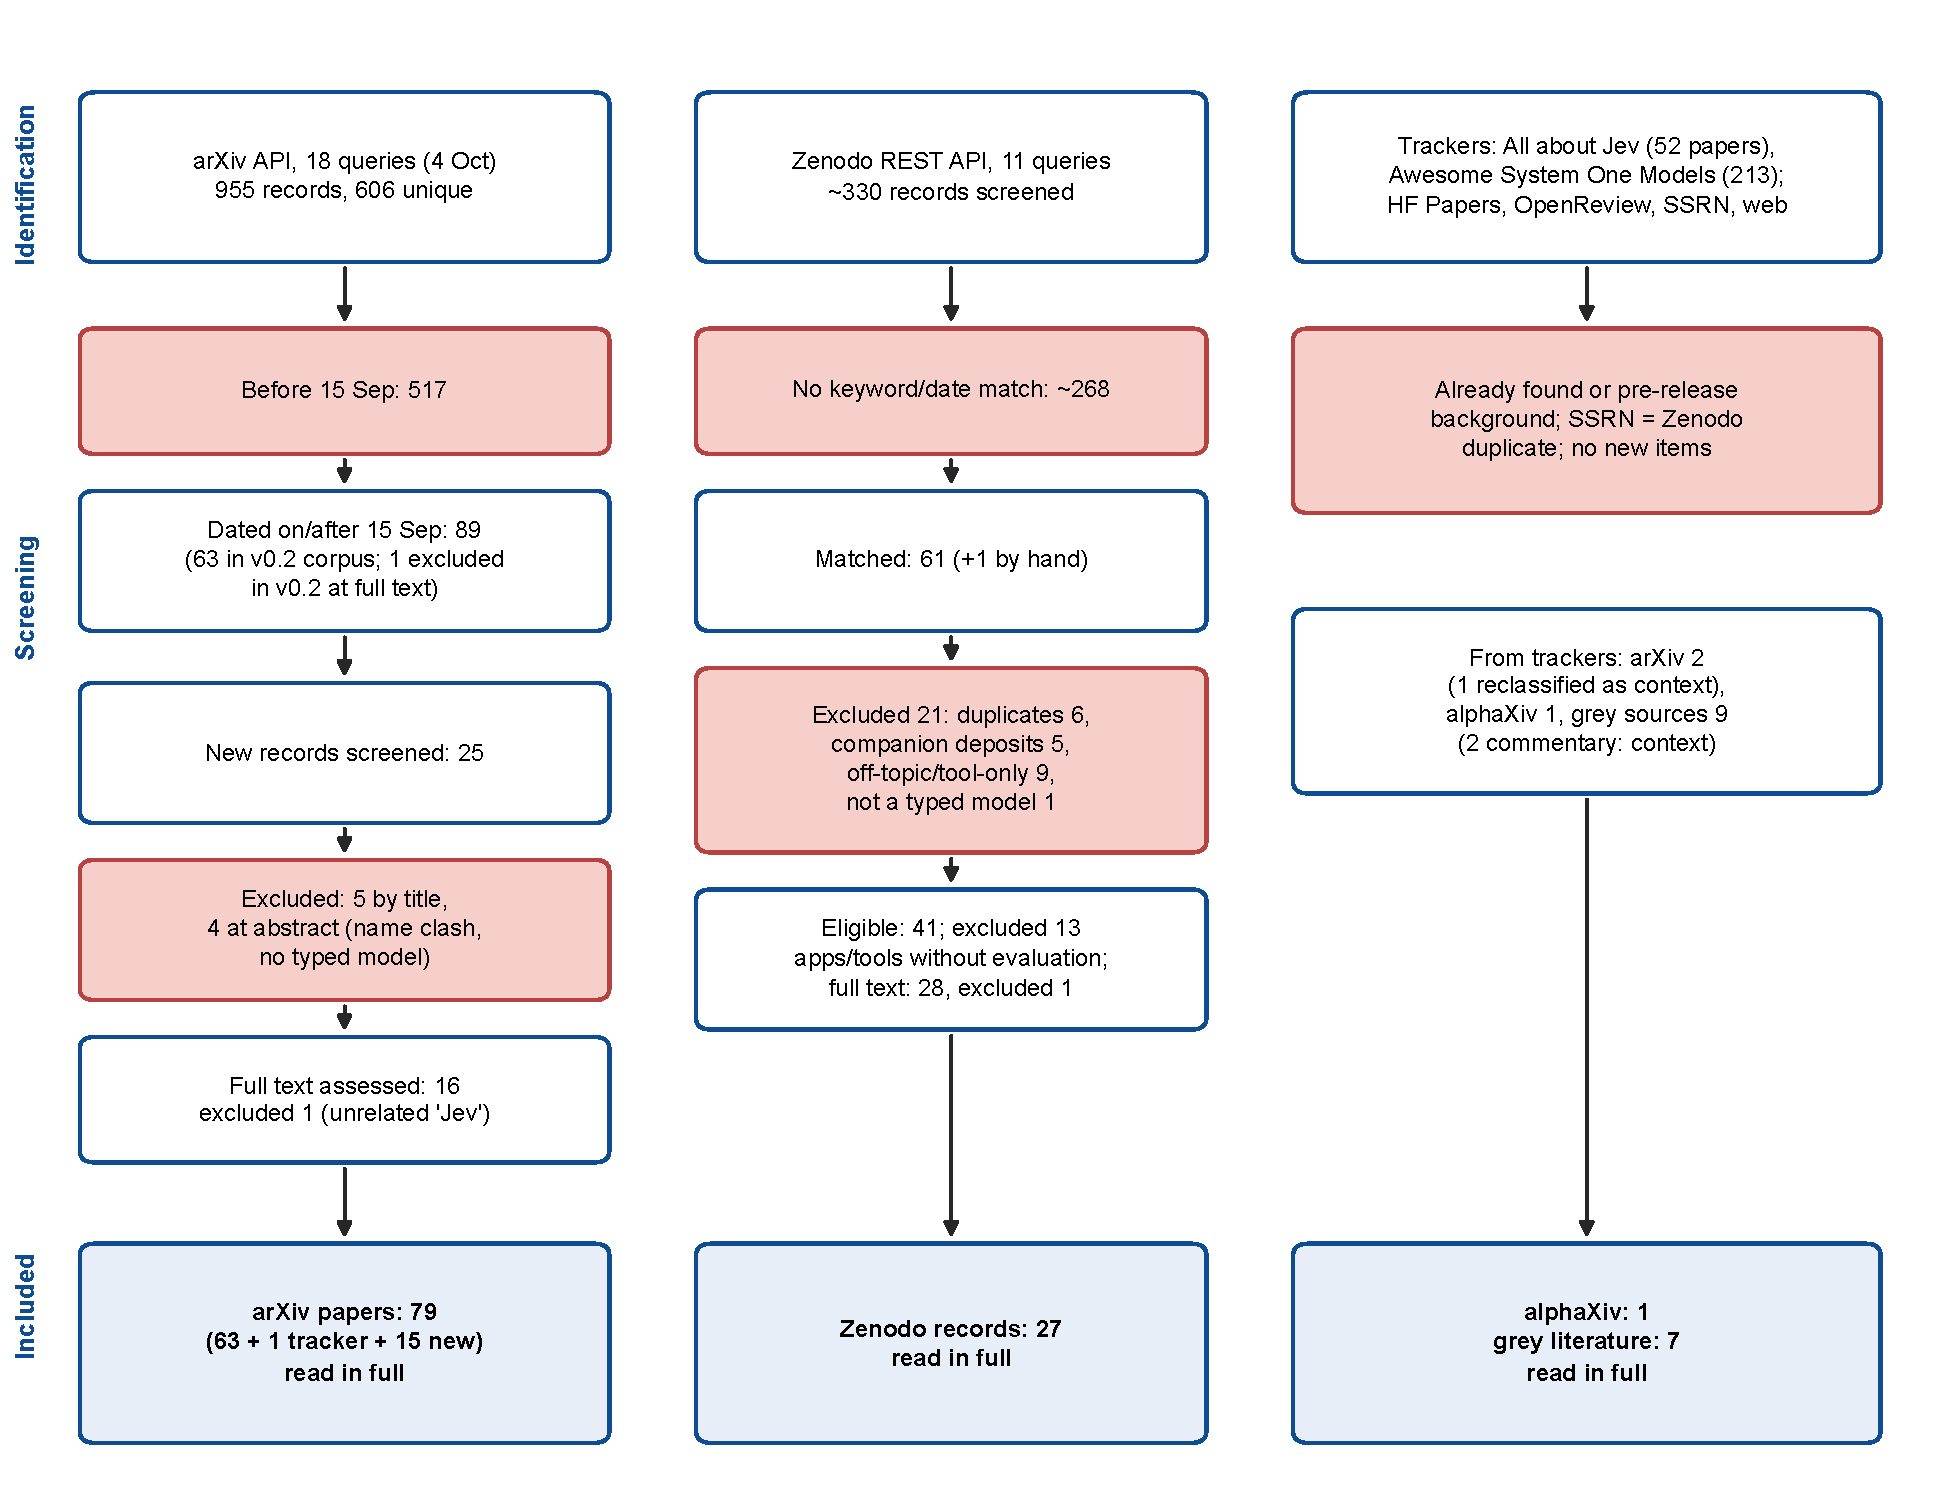
\includegraphics[width=0.85\linewidth]{figures/fig_prisma.pdf}
\caption{Identification, screening and inclusion by source (PRISMA 2020 flow). Zenodo counts at the first step are approximate because the API returns overlapping result sets.}
\label{fig:prisma}
\end{figure}

\paragraph{PRISMA 2020 checklist.}
\Cref{tab:prisma} maps the PRISMA~2020 items~\cite{page2021prisma} to this paper; items that were not done are stated as such.

\begingroup
\small
\renewcommand{\arraystretch}{1.15}
\begin{longtable}{@{}p{0.30\linewidth}p{0.64\linewidth}@{}}
\caption{PRISMA 2020 items and where they are reported.}\label{tab:prisma}\\
\toprule
Item & Where reported, or status \\
\midrule
\endfirsthead
\toprule
Item & Where reported, or status \\
\midrule
\endhead
\bottomrule
\endfoot
Title (1) & Not followed by design: the paper is a policy analysis, and its evidence component is identified as a structured rapid evidence assessment in \cref{sec:method} \\
Abstract (2) & Abstract states question, sources, method, main results, certainty and implications \\
Rationale, objectives (3--4) & \Cref{sec:intro} (research question) \\
Eligibility criteria (5) & \Cref{sec:method}, Eligibility \\
Information sources, search (6--7) & \Cref{sec:method}; \cref{app:queries}; \nolinkurl{scripts/rerun_arxiv_search.py} \\
Selection process (8) & \Cref{sec:method} (Reviewers and tools): AI agents; no duplicate human screening \\
Data collection, items (9--10a/b) & \Cref{sec:method}, Data extraction; \nolinkurl{data/evidence_coding.csv} \\
Study risk of bias (11) & Design appraisal (\cref{sec:appraisal}); \nolinkurl{data/quality_appraisal.csv} \\
Effect measures (12) & Not applicable: direction of the primary result per requirement; no pooled effect \\
Synthesis: eligibility for each synthesis (13a) & Studies coded for a requirement (\cref{app:evidence}) \\
Synthesis: data preparation (13b) & Codes and comparator fields from the extraction; no conversion \\
Synthesis: tabulation and display (13c) & \Cref{fig:framework}, \cref{tab:keyfindings} and \cref{tab:evidence} \\
Synthesis: methods (13d) & Vote counting of direction following SWiM~\cite{campbell2020swim}; no meta-analysis \\
Synthesis: heterogeneity (13e) & Not done formally; heterogeneity of tasks and models is described in \cref{sec:evidence} \\
Synthesis: sensitivity analyses (13f) & Stronger-design studies only; Zenodo records excluded (\cref{sec:across}) \\
Reporting bias (14) & Not formally assessed; discussed in \cref{sec:discussion} \\
Certainty assessment (15) & GRADE-style rules (\cref{sec:appraisal}); \cref{tab:keyfindings} \\
Study selection (16a) & \Cref{fig:prisma} \\
Excluded studies that appear eligible (16b) & \nolinkurl{data/excluded_records.csv} (e.g.\ the unrelated ``Jev'' paper, the mismatched PDF and the harness paper without a typed model) \\
Study characteristics (17) & \Cref{app:evidence,app:catalogue} \\
Risk of bias in studies (18) & \Cref{tab:evidence}; \nolinkurl{data/quality_appraisal.csv} \\
Results of individual studies (19) & \Cref{sec:evidence}; rationales in \nolinkurl{data/evidence_coding.csv} \\
Results of syntheses (20a--d) & \Cref{sec:evidence,sec:across}; \cref{fig:framework}; heterogeneity and formal tests not done \\
Reporting biases (21) & Not assessed formally (\cref{sec:discussion}) \\
Certainty of evidence (22) & \Cref{tab:keyfindings} \\
Discussion (23a--d) & \Cref{sec:discussion} (interpretation, limitations of evidence and of the process, implications) \\
Registration and protocol (24a--c) & Not registered; no protocol published; changes from the earlier release in \cref{sec:method} \\
Support (25) & No funding \\
Competing interests (26) & Positionality and competing interests statement \\
Availability of data, code and materials (27) & Data and code availability statement \\
\end{longtable}
\endgroup


\bibliographystyle{unsrtnat}
\bibliography{pol2,corpus,corpus_update,grey,background}
\end{document}
